% !TEX TS-program = Arara
% arara: pdflatex
% arara: nomencl
% arara: pdflatex
\documentclass[12pt,twoside]{article}
\usepackage[a4paper,width=150mm,top=25mm,bottom=25mm, bindingoffset=6mm]{geometry}

\usepackage[]{biblatex}
\addbibresource{sources.bib}

\usepackage{caption}
\usepackage{subcaption}

\usepackage{listings}
\lstset{language=Python}

\usepackage[hidelinks]{hyperref}


\usepackage{graphicx} 
\usepackage[ngerman]{babel}
\usepackage[utf8]{inputenc}
\usepackage[T1]{fontenc}    
\usepackage{amsmath}
\usepackage{float}
\usepackage{url}
\usepackage{dirtytalk}
\usepackage{makeidx}
\makeindex

\newlength{\swidth}
\setlength{\swidth}{0.6\textwidth}

\pagestyle{plain}

\title{deepLID}
\author{Joel André}
\date{\today{}}

\begin{document}
	
	\begin{titlepage}
    \begin{center}
        \vspace*{1cm}
        
        \Huge
        \textbf{Identifikation gesprochener Sprache mit Deep Learning}
            
        \vspace{4cm}
        
        
\includegraphics[width=0.4\textwidth]{assets/front.png}
        
         \vspace{4cm}
        
        \textbf{Joel André}
        \vspace{2.5cm}
        
        
        \Large
        Maturaarbeit\\
        Betreut von
        Beni Keller
        
        \vspace{0.8cm}
        
        
        Kantonsschule Zug\\
        2019
        
    \end{center}
\end{titlepage}
	
	\tableofcontents
	\newpage
	
	\section{Einleitung}
Sprachoberflächen sind der aktuelle Megatrend in der Tech-Branche. Ein Algorithmus, der natürliche Sprache zuverlässig versteht, ist längst kein Science-Fiction mehr. High-Tech-Firmen rund um den Globus investieren Milliarden in die Entwicklung solcher Produkte. Genau wie das iPhone mit dem Touchscreen eine Revolution der Interaktion Mensch-Maschine lancierte, erhofft man sich mit Spracherkennung den nächsten Durchbruch. Sprachgesteuerte Programme sollen weitaus intuitiver zu bedienen sein als Texteingaben. In Zukunft ist die lästige Uhrzeitabfrage-Bewegung zum Handy wahrscheinlich Geschichte. Wir werden bequem danach fragen können.
\\ \\
Moderne Spracherkennung-Systeme sind auf einzelne Sprachen spezialisiert. Aus diesem Grund muss ein sprachunabhängiges System, in erster Linie die verwendete Sprache identifizieren, um anschliessend, den passende Sprachassistenten anzuwenden. Der sprachabhängige Sprachassistent kann dann zum Beispiel die Grammatik der erkannten Sprache zur Hilfe nehmen, um nur grammatikalisch korrekte Sätze zu erkennen. In dieser Arbeit geht es darum den Prozess der Sprachidentifikation zu implementieren:  Aufnahmen mündlicher Äusserungen sollen der korrekten Sprache zugeordnet werden. 
\\ 
Die Idee zu diesem Thema entstand spontan. Für mich war aber seit Anfang an klar, dass ich meine Maturaarbeit im Fach Informatik schreiben wollte. Ich nahm bereits an der Informatikolympiade und dem Freifach \textit{Begabtenförderung Informatik} teil. Mich weiter in diesen Bereich zu vertiefen, war eine logische Konsequenz. Überdies besitzen die meisten Informatik-Projekte den Vorteil äusserst ressourcenarm zu sein. Ein Computer mit Internet-Anschluss reicht, um ein innovatives Produkt zu entwickeln, dass die Welt verändern kann. Das nötige Wissen lässt sich ohne lange Ausbildung im Internet finden. Entsprechend erlaubt Informatik Jugendlichen, bereits Teil der Wirtschaft zu sein. Kein 14-Jähriger kann, ohne teures Labor Medikamente entwickeln, hingegen für die Idee \textit{Blockchain} hätte theoretisch jeder die Mittel gehabt.
\\ \\
Für die Sprachidentifikation verwende ich in dieser Arbeit die Methode \textit{Künstliche Intelligenz} (KI). KI ist ein prominentes junges Teilgebiet der Informatik. In den letzten Jahren wurden enorme Fortschritte gemacht, was dazu führt, dass die Wirtschaft der Forschung weit hinterherhinkt. Dank fortgeschrittener Computer-Hardware und neuen Algorithmen können Maschinen heute Aufgaben lösen, die vor zehn Jahren unmöglich erschienen.
Mittlerweile sind zum Beispiel sogar selbst-fahrende Autos nur noch eine Frage der Zeit. Dem Traum der Menschen, eine ihr in Intelligenz ebenbürtige Maschine zu entwerfen, kommt man langsam aber stetig näher.
\\
Die klassischen Projekte in KI-Arbeiten sind oft Spiele. Es wird dem Computer beigebracht besser zu spielen als jeder Mensch. So ist es zum Beispiel beim Schachcomputer
\textit{Deep blue}\parencite{deepblue} , dass 1996 Garry Kasparov schlug, oder dem Go-Programm \textit{AlphaGo}\parencite{alphago}.
Solche Projekte bieten zwar gute Forschungsobjekte, sind aber an sich keine Anwendungsfelder. Ich wollte in meiner Arbeit etwas programmieren, das tatsächlich einen realen Nutzen
besitzt.
Sprachidentifikation erfüllt das Kriterium. Sprachidentfikation kann nebst für die Spracherkennung, unter anderem im Anrufcenter angewendet werden. Ein Computer erkennt die Sprache des Kunden und leitet den Anruf an den passenden Mitarbeiter weiter.
\\ \\
Klassische Methoden für die Sprachidentifikation beruhen stark auf Expertenwissen. Analytisch entwickelte, handprogrammierte Verfahren erreichen mit wenig maschinellem Lernen sehr gute Leistungen. In dieser Arbeit wird ein anderer Ansatz gewählt. Der Computer soll möglichst viel selbst erlernen. Aus diesem Grund verwende ich die Technologie \textit{Deep Learning}. 
\\ 
Das Ziel dieser Arbeit lässt sich in zwei Teile gliedern. Zuerst soll KI bzw. Deep Learning beschrieben und soweit wie möglich ein Verständnis dafür geschaffen werden.
Anschliessend wird die Technologie auf das Problem Sprachidentifikation angewendet. Als zu identifizierende Sprachen gelten Französisch, Englisch und Deutsch. Es
werden verschiedene Ansätze probiert und verglichen. Das Produkt soll eine möglichst grosse Fehlerfreiheit besitzen. Um das Produkt zu demonstrieren, wird ein Web-Interface
entwickelt, das einem ermöglicht, das Produkt selber zu testen.
\\ \\
Um die Realisierbarkeit dieses Vorhabens zu beurteilen, hatte ich im Vorfeld der Arbeit, bereits das Buch  \textit{Neuronale Netze selbst programmieren}\parencite{neuronale_netze} aus dem Info-Z gelesen. Dies ermöglichte mir erst, die Fragestellung genauer einzuschränken und den nötigen Aufwand dafür abzuschätzen. Die enthaltenen Informationen waren aber noch lange nicht ausreichend, um mit dem Programmieren zu beginnen. Ausschlaggebend war erst später das Buch \textit{Deep Learning with Python}\parencite{chollet}, das als theoretische Grundlage dient. 
\\
Parallel dazu wurde begonnen, das Web-Interface zu entwickeln. Das nötige Know-How besass ich bereits grösstenteils als Vorwissen. Das dann realisierte Interface erlaubte mir, das Produkt in der Entwicklungsphase live zu testen. 
\\
Der nächste Schritt war endlich das Programmieren am Produkt. In dieser Phase gab das Paper \textit{Practical Applications of Multimedia Retrieval. Language Identification in Audio
Files}\parencite{iLID} die Richtung vor. 
Um die Unterschiede zwischen den Sprachen zu erlernen, benötigt mein Programm viele Trainings-Daten. Die Beschaffung dieser grossen Menge Daten und das effiziente Umgehen damit, sind ein nicht zu unterschätzender Aufwand. 
\\
Die letzte Phase, das Entwickeln der künstlichen Intelligenz, war am spannendsten. Die Komplexität des Themas erlaubte allerdings oft nur oberflächlich, ein Verständnis zu entwickeln, zumal die mathematischen Grundlagen auf Universitäts- Stufe fehlten. 
\\ \\
Im Kapitel \textbf{2 Deep Learning} beschreibe ich kurz die theoretischen Grundlagen zur künstlichen Intelligenz. Das Kapitel bildet das Herz des theoretischen Teils. Das Kapitel \textbf{3
Daten} befasst sich mit den Quellen der Daten, den Methoden zur Datenbeschaffung und den Algorithmen zur Datenbearbeitung. Anschliessend werden in Kapitel \textbf{4 Modelle} die entwickelten KI-Modelle präsentiert. Kapitel \textbf{5 Umsetzung und Resultate} erläutert die Implementierung des Systems und zeigt die Auswertung der Modelle. In \textbf{6 Diskussion} werden die
Ergebnisse in Zusammenhang gestellt und Kapitel \textbf{7 Anhang} gibt Interessierten einen Einblick in einen Teil des Codes. Der Vollständige Programmiercode der Arbeit ist online hier verfügbar: \url{https://github.com/jotron/deepLID}

	\section{Deep learning}
Die Begriffe \textit{Deep Learning}, \textit{maschinelles Lernen} und \textit{künstliche Intelligenz} werden oft fälschlicherweise auswechselbar verwendet. Es gibt allerdings eine ganz klare, und für das Verständnis wichtige Hierarchie zwischen den Wörtern. Um Klarheit zu verschaffen werden darum alle Gebiete aufgeführt.

\begin{figure}[hbt]
	\centering
		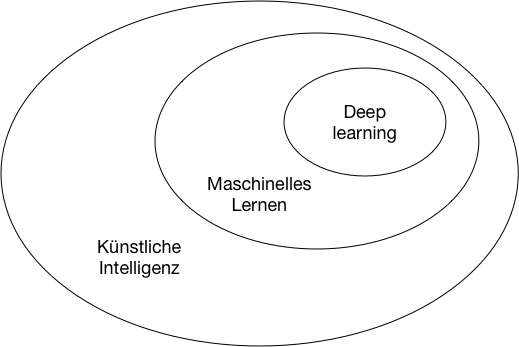
\includegraphics[width=0.6\textwidth]{assets/hierarchy.png}
	\caption{Künstliche Intelligenz, Maschinelles Lernen und Deep Learning}
	\label{img:hierarchy}
\end{figure}

Das Gebiet der künstlichen Intelligenz gibt es schon so lange wie den Computer selbst. Die Frage, wie schlau ein Computer werden kann, beschäftigt uns bis heute. Als anerkannte Definition für KI gilt, das Bestreben intellektuelle Aufgaben, die normalerweise von Menschen gelöst werden, zu automatisieren.\index{Künstliche Intelligenz (KI)}

Erste Erfolge erreichte man zum Beispiel mit Schachcomputern, die handgeschriebene Regeln befolgten. Diese Form von künstlicher Intelligenz hat aber schnell Grenzen, da viele Prozesse schlicht zu komplex sind, um sie unter angemessenem Aufwand mit Regeln zu beschreiben. Um dieses Problem zu lösen, erfand man maschinelles Lernens. \index{Maschinelles Lernen}

Der Ablauf von maschinellem Lernen ist grundlegend anders als konventionelles Programmieren. Der Entwickler muss  keinen Programmcode mit festen Regeln schreiben, im Gegenteil: Er liefert dem Computer Eingabe und Ausgabe, und der Computer lernt die Regeln selbst. Kurzgesagt lernt das System aus Beispielen Muster zu erkennen. Maschinelles Lernen blühte erst in den 90'er Jahren auf, wurde aber schnell zum grössten Teilgebiet der künstlichen Intelligenz.

Beim maschinellem Lernen, lernt die Software im Grunde eine nützlichere Darstellungsweise der Daten bzw. der Eingabe. Anhand dieser anderen Darstellungsweise kann der Computer die Antwort einfach erkennen. Wenn der Computer stufenweise nützlichere Repräsentationen bestimmt, kann er zunehmend komplexe Probleme, in einfacheren Zwischenschritten lösen. Genau das ist \textit{Deep Learning}. Das \textit{Deep} entspringt der grossen Anzahl an aufeinanderfolgenden Repräsentation. Deep Learning bezeichnet das Konzept von stufenweisem Lernen und nicht eine Methode selbst. Eine weit verbreitete Methode sind allerdings \textit{tiefe künstliche neuronale Netze}.\parencite[vgl.][]{chollet} \index{Deep Learning}

\subsection{Künstliche neuronale Netze}

\textit{Künstliche neuronale Netze} \index{Künstliche neuronale Netze}hat man sich, wie der Name schon preisgibt, von der Natur abgesehen. Ähnlich wie in unserem Gehirn gibt es Neuronen bzw. Knoten und dazwischenliegende Verbindungen. Die \say{Intelligenz} entsteht erst aus dem Zusammenspiel tausender Neuronen. Künstliche Neurone Netze haben sich mittlerweile so stark weiterentwickelt, dass sie nebst der ursprünglichen Idee, nichts mehr mit der biologischen Variante gemeinsam haben. \\

Der Wert eines Knotens/Neurons ist abhängig von der Summe aller seiner eingehenden Verbindungen. Die Abhängigkeit wird duch die Aktivierungsfunktion $\sigma$ definiert. Die Aktivierungssfunktion ist wichtig, damit das Netzwerk jede mögliche Funktion abbilden kann. Es ist bewiesen dass neuronalen Netze universelle Approximatoren sind\parencite[][Kap. 4]{universal}. Eine bekannte Aktivierungsfunktion ist zum Beispiel die \textit{ReLU} \index{ReLU}Funktion. Die ReLU Funktion unterdrückt negative Werte, bzw. sie ist null für Werte kleiner als null.   \parencite{neuronale_netze} 
$$\sigma(x) = \text{ReLU}(x) = \text{max}(0, x)$$

Der Wert einer eingehenden Verbindung ist proportional zum Wert des Herkunfsknoten, bzw. des Knoten woher die Verbindung kommt. Der Wert des Herkunfsknoten wird multipliziert mit dem Gewicht der Verbindung: $w$. Die Gewichte der Verbindungen sind die Parameter des Netzwerks. Intuitiv kann man sich vorstellen, dass das Netzwerk lernt, wichtigeren Verbindungen grössere Gewichte zuzuordnen und Unwichtigen umgekehrt. Wenn man alles zusammensetzt ergibt sich für den Wert irgendeinen Knotens $o_i$ mit Vorgänger-Knoten $\boldsymbol{h}$ diese Formel:
$$ o_i = \sigma\Big(\sum_i h_i \cdot w_{i}\Big)$$
Mit dieser Formel propagieren sich die Werte der Anfangsknoten durch das ganze Netzwerk. Um das Prinzip anschaulicher zu machen, wird ein Beispiel-Durchlauf vorgeführt. Die verwendeten Gewichte und Eingaben sind willkürlich.

Die Aufgabe des vorgestellten Netzwerks ist es zum Beispiel, zwischen Hund und Katze zu unterscheiden. Die Eingaben $x_1$ und $x_2$ sind gewisse Merkmale des zu erkennenden Tieres. $1$ bedeutet, dass Tier besitzt das Attribut und $0$ das Gegenteil. Die Ausgabe $o$ beschreibt die Wahrscheinlichkeit, dass das Tier eine Katze ist. Daraus folgt, dass Werte $o>0.5$ für Katze stehen und Werte $o<0.5$ für Hunde.
\begin{figure}[hbt]
	\centering
		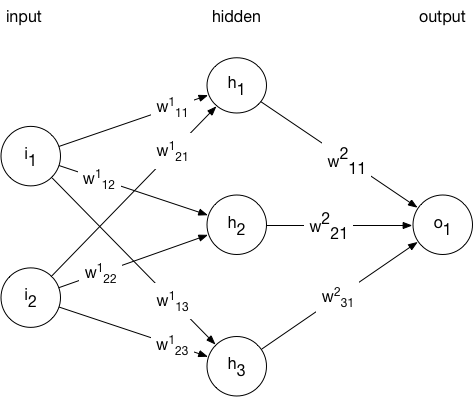
\includegraphics[width=0.85\textwidth]{assets/neural_net.png}
	\caption{Grafische Darstellung eines künstlichen neuronalen Netzwerks anhand eines Beispiels: Rote Zahlen sind festgesetzt und grüne Zahlen werden berechnet.}
	\label{img:neuralnet}
\end{figure}

Was bis jetzt berechnet wurde nennt man den \textit{Vorwärtspass}. Aus einer Eingabe wurde die Ausgabe berechnet. Daran war aber noch nichts intelligent. Erst jetzt können die Parameter der Funktion, die Gewichte, aus diesem Beispiel lernen (Siehe Abbildung \ref{img:anatomy}). Um diese zu verbessern braucht es eine \textit{Verlust Funktion} \index{Verlust Funktion}die uns angibt, wie weit die Ausgabe vom korrekten Ziel entfernt ist. Eine mögliche Verlust Funktion ist die absolute Differenz zwischen dem Ziel und der Ausgabe. Wenn man in oberen Beispiel davon ausgeht, dass die Eingabe wirklich zu einer Katze gehört, ergäbe sich:
$$ \text{Verlust}(output, target) = |target-output| = |1.0-0.747| = 0.253$$
Um den Verlustwert zu minimieren, passt das Netzwerk die Gewichte schrittweise an. Diesen Teil übernimmt der  \textit{Optimierer}. Ein einfacher Optimierer ist zum Beispiel das Gradientenverfahren. Details dazu befinden sich in \parencite{gradient}.

\begin{figure}[hbt]
	\centering
		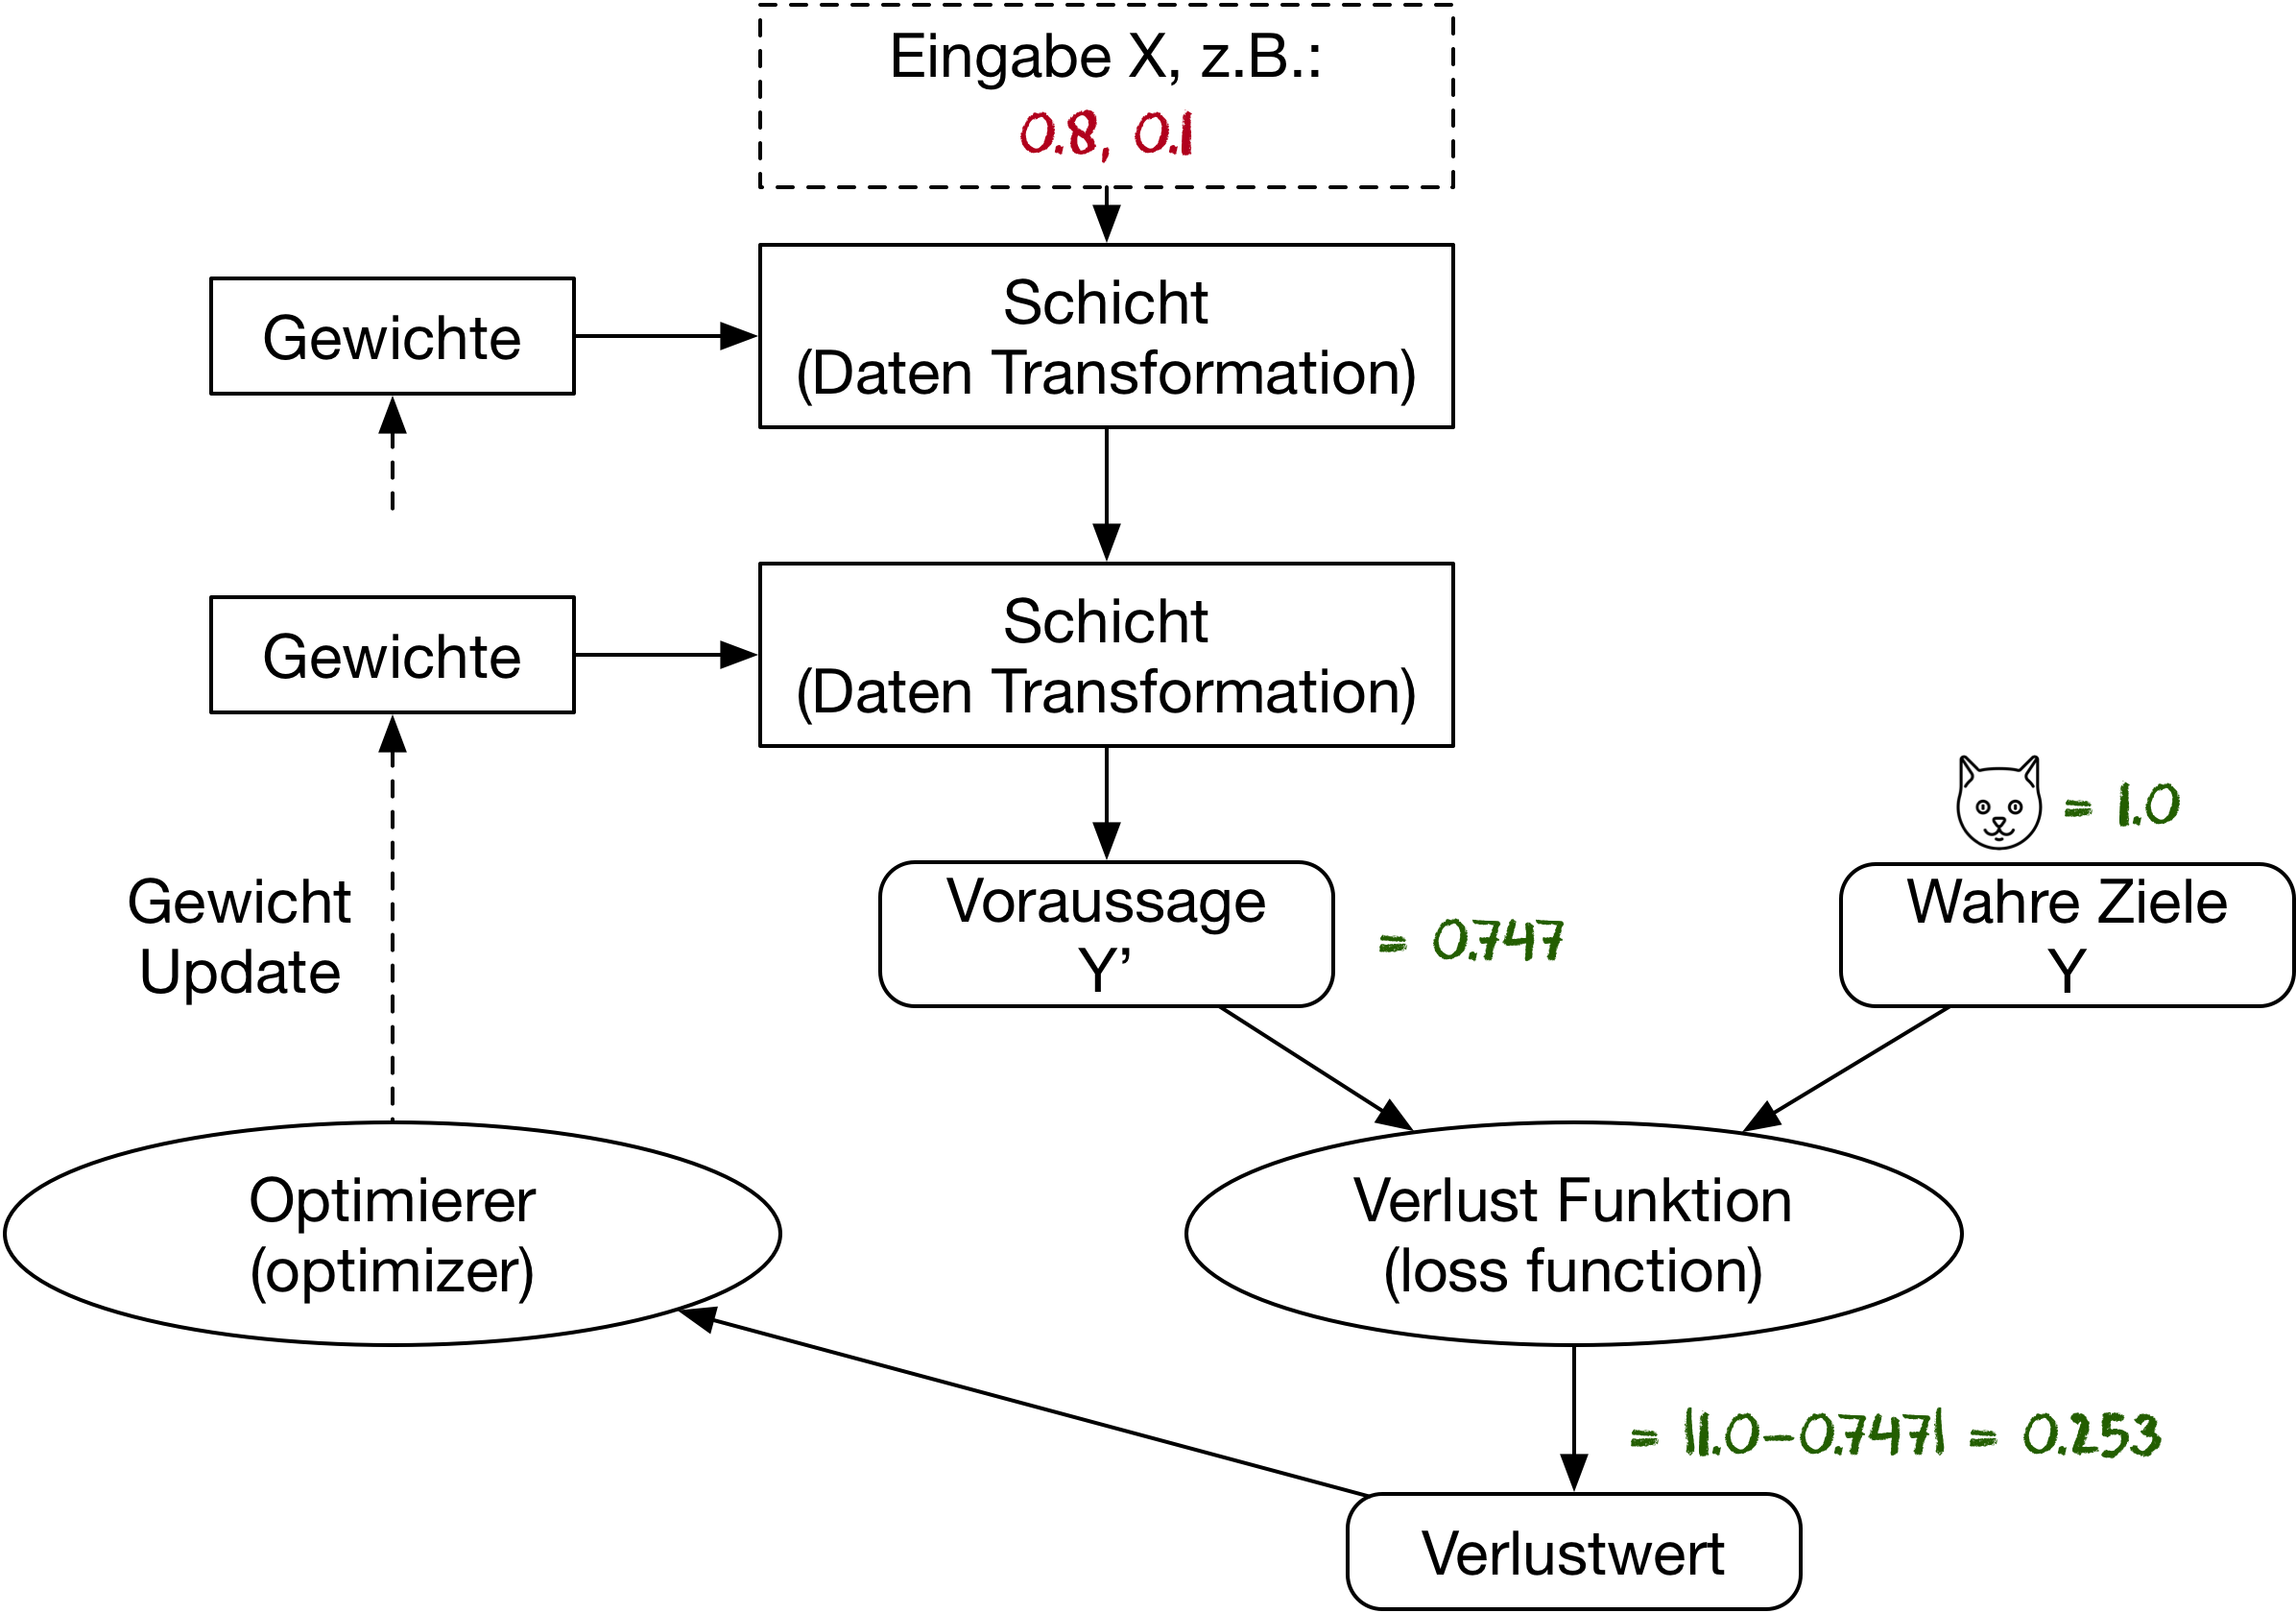
\includegraphics[width=0.8\textwidth]{assets/anatomy.png}
	\caption{Visuelle Darstellung des Lern-Prozesses anhand eines Beispiels}
	\label{img:anatomy}
\end{figure}

Da bei diesem Typ von neuronalen Netzwerken alle Knoten miteinander verbunden sind, wird es oft \textit{Dense Neural Network} \index{Dense Neural Network}genannt.
\\
Die mathematischen Operationen in einem neuronalen Netzwerk lassen sich alle als Matrizen-Operationen berechnen. Mit Matrizen kann der Computer auf einer Grafikkarte und mit einem BLAS \index{BLAS}(\textit{Basic linear algebra system}) sehr effizient rechnen \parencite{neuronale_netze} .


\subsection{Convolutional Neural Networks}
\textit{Convolutional Neural Networks} \index{Convolutional Neural Networks (CNN)}sind eine sehr weit verbreitete Methode im Feld von \textit{Computer Vision}. Der fundamentale Unterschied zwischen dem oben besprochenen \textit{dense network} und einem \textit{CNN} ist, dass ein \textit{CNN} lokale Muster erkennen kann, wo hingegen das vorherige Netzwerk nur globale Muster erkennen konnte. Das bedeutet, dass ein Muster, das an einer bestimmten Stelle angetroffen wird, an jeder anderen Stelle ebenfalls erkannt wird. \parencite{chollet}

Um das zu erlauben, teilen gewisse Verbindungen das gleiche Gewicht. In Abbildung \ref{img:conv} (Oberer Teil) sind das die gleichfarbigen Verbindungen. Weniger Gewichte führen zusätzlich dazu, dass das Netzwerk schneller lernen kann.
\begin{figure}[hbt]
	\centering
		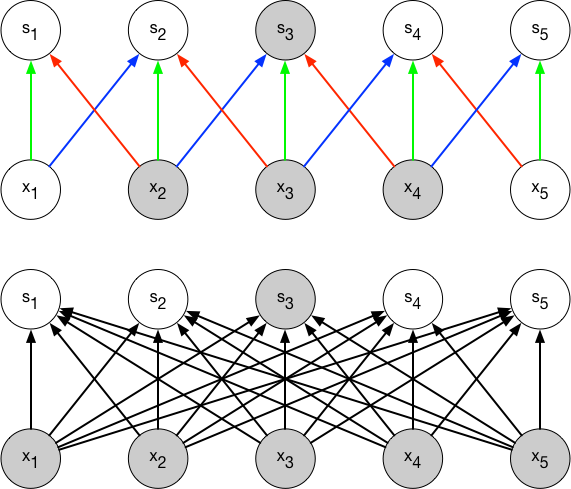
\includegraphics[width=0.6\textwidth]{assets/conv_1d.png}
	\caption{(\textit{Oben})1D Convolution mit \textit{kernel} der Grösse 3. $s_3$ wird durch 3 inputs beeinflusst.
		     (\textit{Unten}) \textit{Dense Network}. $s_3$ wird durch alle inputs beeinflusst.\parencite{goodfellow}}
	\label{img:conv}
\end{figure}

Ein weiterer Vorteil von \textit{Convolutional Neural Networks} ist, dass sie eine räumliche Hyrarchie von Mustern erlernen können. Wenn die Eingabe das Bild einer Katze ist, wird zum Beispiel die erste Schicht unterschiedliche Kanten erkennen, die zweite Schicht dann einzelne Merkmale (z.b Augen), und so weiter.

Damit das gilt, muss aber der analysierte Bereich eines Knotens, von Schicht zu Schicht grösser werden. Deshalb wird meisten nach jedem \textit{Convolution Layer} ein \textit{Pooling Layer} gesetzt. Das \textit{Pooling Layer} fasst mehrere Datenpunkte zusammen um dem nächsten Netzwerk eine grösseren Analysebereich zu verschaffen. Ein oft verwendetes Pooling-Verfahren ist \textit{Max-Pooling}: Angrenzende Knoten werden zusammengefasst durch ihr Maximum. \index{Max-Pooling}
\begin{figure}[hbt]
	\centering
		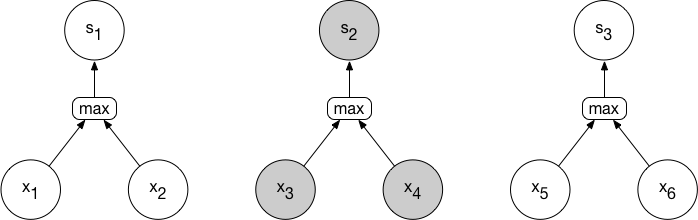
\includegraphics[width=0.75\textwidth]{assets/pooling_1d.png}
	\caption{1D Max-Pooling layer: z.B $s_2$ ist $\max (x3, x4)$}
	\label{img:pool}
\end{figure}


\subsection{Recurrent Neural Networks}
Eine gemeinsame Eigenschaft von allen \textit{Dense Neural Networks} und CNN's ist, dass sie keinen Speicher haben. Bei jedem Vorwärtspass berechnet das Netzwerk alles von neuem ohne Erinnerungen an vorherige Durchlaufe. Dieses Verhalten ist das absolute Gegenteil vom menschlichem Denkprozess. Wenn wir einen Satz lesen, durchgehen wir ihn Wort nach Wort und merken uns den vorherigen Kontext.

\textit{Recurrent Neural Networks} (RNN) bilden diesen Prozess vereinfacht nach. Sie besitzen eine interne wiederkehrende Schleife die dem Netzwerk Informationen aus dem vorherigen Durchlauf bereitstellt (Siehe Abbildung \ref{img:rnn_loop}). Die RNN Zelle berechnet dann die nächste Ausgabe sowohl aus der neuen Eingabe, wie auch mit den Erinnerungen der letzten Ausgabe. \parencite{chollet}\\
\begin{figure}[hbt]
	\centering
		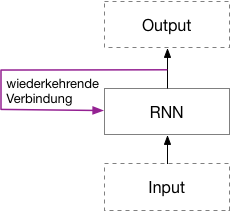
\includegraphics[width=0.35\textwidth]{assets/rnn_loop.png}
	\caption{RNN mit Schlaufe}
	\label{img:rnn_loop}
\end{figure}

Der Vorgang lässt sich grafisch über die Zeit aufgerollt darstellen (Abbildung \ref{img:rnn_unrolled}). In dieser Darstellung fällt auf, dass das Netzwerk theoretisch für jeden Schritt eine Ausgabe besitzt. Die zwischenliegenden Ausgaben sind vor allem wichtig, wenn man eine weitere Schicht an das Netzwerk anhängen will. Sonst behält man meist nur die letze Ausgabe, da diese indirekt Informationen über alle anderen beinhaltet.\\
\begin{figure}[hbt]
	\centering
		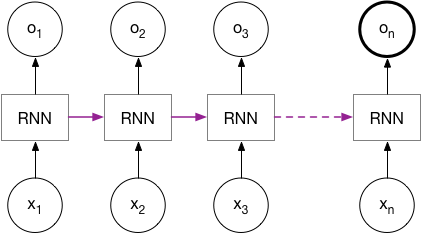
\includegraphics[width=0.67\textwidth]{assets/rnn_unrolled.png}
	\caption{RNN aufgerollt über die Zeit}
	\label{img:rnn_unrolled}
\end{figure}

Das ganze Prinzip ergibt jedoch nur Sinn, wenn frühere Eingaben tatsächlich einen Einfluss auf spätere Ausgaben haben. Eine praktische Anwendung ist das Verarbeiten von zeitlichen Sequenzen wie Wetterdaten und Sprache. Die einzelnen Lernbeispiele werden  zeitlich zerteilt und stückweise dem Netzwerk gefüttert.
Eine fortgeschrittene Implementation von RNN Zellen ist unter anderem die \textit{Long short-tem memory} (LSTM) Zelle \parencite{schmidhuber}. Durch das Einführen von unterschiedlichen wiederkehrenden Verbindungen wird verhindert, dass ältere Signale langsam verschwinden, bzw. vergessen werden \parencite{chollet}.
	\section{Daten}


\subsection{Datenquellen}
Es gibt keine frei zugänglichen umfassenden Datensets für Sprachidentifikation. Datensets wie das \textit{NIST Language Recognition Evaluation}\cite{nist} sind nur unter teuren Gebühren zugänglich. Wie verwandte Arbeiten empfehlen \cite{iLID}, wird darum ein eigenes Datenset zusammengestellt. Es werden gleichmässig Daten zu den Sprachen Deutsch, Englisch, und Französisch gesammelt. Die Daten stammen vom \textit{Voxforge}\cite{voxforge} Datenset, von \textit{Youtube}\cite{youtube} und von \textit{Librivox}\cite{librivox}.

\paragraph{Voxforge} ist ein open-source Datenset für Spracherkennung. Es besteht aus vielen kurzen (1-10s), von Benutzern hochgeladenen, Audiodateien. Die englische Sprache dominiert mit rund 120h Audio das Datenset. Über alle drei Sprachen verteilt sind 190 Stunden Ton verfügbar. Die Audioqualität variiert je nach Benutzer.

Die Sprache ist langsam und deutlich verständlich. Sie hört sich eher künstlich an im Vergleich zu einem natürlichem Gespräch. Die Anzahl unterschiedlicher Sprecher ist gering.

\paragraph{Youtube}dient als Quelle für abwechslungsreiche Sprache. Es werden populären Nachrichtenkanäle wie CNN, ARD, etc. verwendet (Siehe Tabelle \ref{tab:channels}). Die Aufnahmen werden oft von diversen Hintergrundgeräuschen begleitet und die Variation der Sprecher gross, da oft fremde Gäste eingeladen werden. Kehrseite ist, dass nicht garantiert werden kann, dass alle Aufnahmen tatsächlich die richtige Sprache beinhalten. Sendepausen und fremdsprachige Interviews kommen vereinzelt vor.
\begin{table}[h]
        \centering
        \begin{tabular}[t]{l || l}
        Sprache & Kanäle \\
        \hline \hline
        Französisch & France24, FranceInfo\\
        Deutsch & ARD, ZDF\\
        Englisch & CNN,  BBC
        \end{tabular}
        \caption{Youtube Kanäle}
        \label{tab:channels}
\end{table}

\paragraph{Librivox} ist ein öffentlich abrufbares Hörbuch Datenset. Anstatt selbst Hörbücher zu selektieren, wird eine vorgefertigte Selektion verwendet \cite{librivox-compilation}. Verfügbar sind sieben Stunden Aufnahmen mit 90 verschiedenen Sprechern.


\subsection{Daten Auswahl}
Die Modelle werden grundsätzlich mit den Daten von Voxforge und Youtube trainiert und ausgewertet. Es werden zwei unterschiedliche Datenquellen verwendet um die \textit{Stichprobenverzerrung} zu minimieren. Stichprobenverzerrung bedeutet, dass das Datenset nicht repräsentativ für alle Sprachaufnahmen ist. Bei Voxforge ist zum Beispiel die Gefahr, dass das Modell sich überanpasst an die geringe Anzahl Sprecher. Anstatt die Sprache zu erkennen, könnte das Modell das Mikrofon des Sprechers identifizieren und jedem Sprecher eine Sprache zuordnen. Die Leistung des Modells für neue Sprecher wäre dann nicht besser als ein Zufallsgenerator.
\\
Um die Stichprobenverzerrung zu messen werden die Modelle zusätzlich auf dem Librivox Datenset ausgewertet. Die Daten von Librivox teilen keine systematischen "Fehler" wie zum Beispiel Sprecher mit den Trainingsdaten. Das Librivox-Testset besteht aus insgesamt 2 Stunden Aufnahmen.
\\
Von Youtube und Voxforge werden gemeinsam 139 Stunden Audiodaten heruntergeladen, was 100'000 5s Aufnahmen entspricht. Die Datenmenge wird bewusst klein gehalten, weil grössere Datenmengen ressourcenaufwändiger und ineffizienter wären. Die einzelnen Sprachen und Quellen sind zu gleichen Teilen repräsentiert. 
\\
Die Daten werden weiter in 80\% Trainingsdaten, 10\% Testdaten und 10\% \textit{Validationset} gespalten. Das Validationset wird verwendet um während dem Training zu beobachten, wie das Modell auf neue Daten reagiert. Die \textit{Hyperparamter} \index{Hyperparameter}(Parameter die das Netzwerk nicht selber lernen kann, z.B die Anzahl Knoten) werden manuell so angepasst dass das Netzwerk möglichst gut auf dem Validationset abschneidet. Tabelle \ref{tab:data} gibt eine Übersicht über die Verteilung der Daten.
\begin{table}[]
	\centering
	\begin{tabular}{llll}
	\hline
	Netz          & Voxforge & Youtube & Librivox \\ \hline
	Trainingset   & 56h      & 56h     & -        \\
	Validationset & 7h       & 7h      & -        \\
	Testset       & 7h       & 7h      & 2h       \\ \hline
	\end{tabular}
	\caption{Daten Verteilung}
	\label{tab:data}
\end{table}


\subsection{Preprocessing}
Sprache besteht aus Wörtern und Wörter sind grundsätzlich eine Abfolge von Lauten. Verschiedene Sprachen unterscheiden sich an den verschiedenen Abfolgen von Lauten, manchmal sogar an den verwendeten Lauten selbst. Die kleinste relevante Einheit für Spracherkennung, sowohl für den Menschen wie die Maschine, ist also ein Laut.

Wenn der Computer mit dem Mikrofon aufnimmt, misst er kleinste Druckunterschiede, bzw. Schallwellen. Eine unkomprimierte Audiodatei zeigt den Schalldruck über die Länge der Aufnahme, siehe Abbildung \ref{img:preprocessing} \textit{(oben)}.
Die einzelne Schallwelle ist für den Menschen nicht erkennbar, deshalb ist sie auch für die Sprache von keiner Bedeutung. Erst mehrere Schallwellen, bzw. die daraus folgende Frequenz lässt sich als Laut hören. 

Das Verfahren um aus einer Schallwelle die unterschiedlichen Frequenzen zu bestimmen heisst \textit{Fourier-Transformation} \cite{fourrier}. Falls dem Netzwerk als Eingabe rohe Schallwellen gefüttert werden, muss es dieses Verfahren erlernen, um dann aus den Lauten die Sprache erkennen zu können. Allerdings ist die Fourrier-Transformation zu erlernen ein zusätzlicher Aufwand und fordert den Computer darum mehr. Um dem Algorithmus die Aufgabe zu erleichtern, kann man ihm darum als Eingabe die berechneten Laute anstatt der rohen Schallwelle geben.

Die Prozedur dem Algorithmus bereits vorgerechnete Werte zu füttern, heisst \textit{Preprocessing} \index{Preprocessing}und ist weit verbreitet im Feld von \textit{Machine learning}. Das Vorrechnen ist unter dem Namen \index{Feature Engineering}\textit{Feature Engineering} bekannt. \textit{Features}, also Merkmale z.b Laute werden aus den Rohen Daten extrahiert. \parencite[vgl.][]{chollet}

\subsubsection{Spektrogramme}
\begin{figure}[hbt]
	\centering
		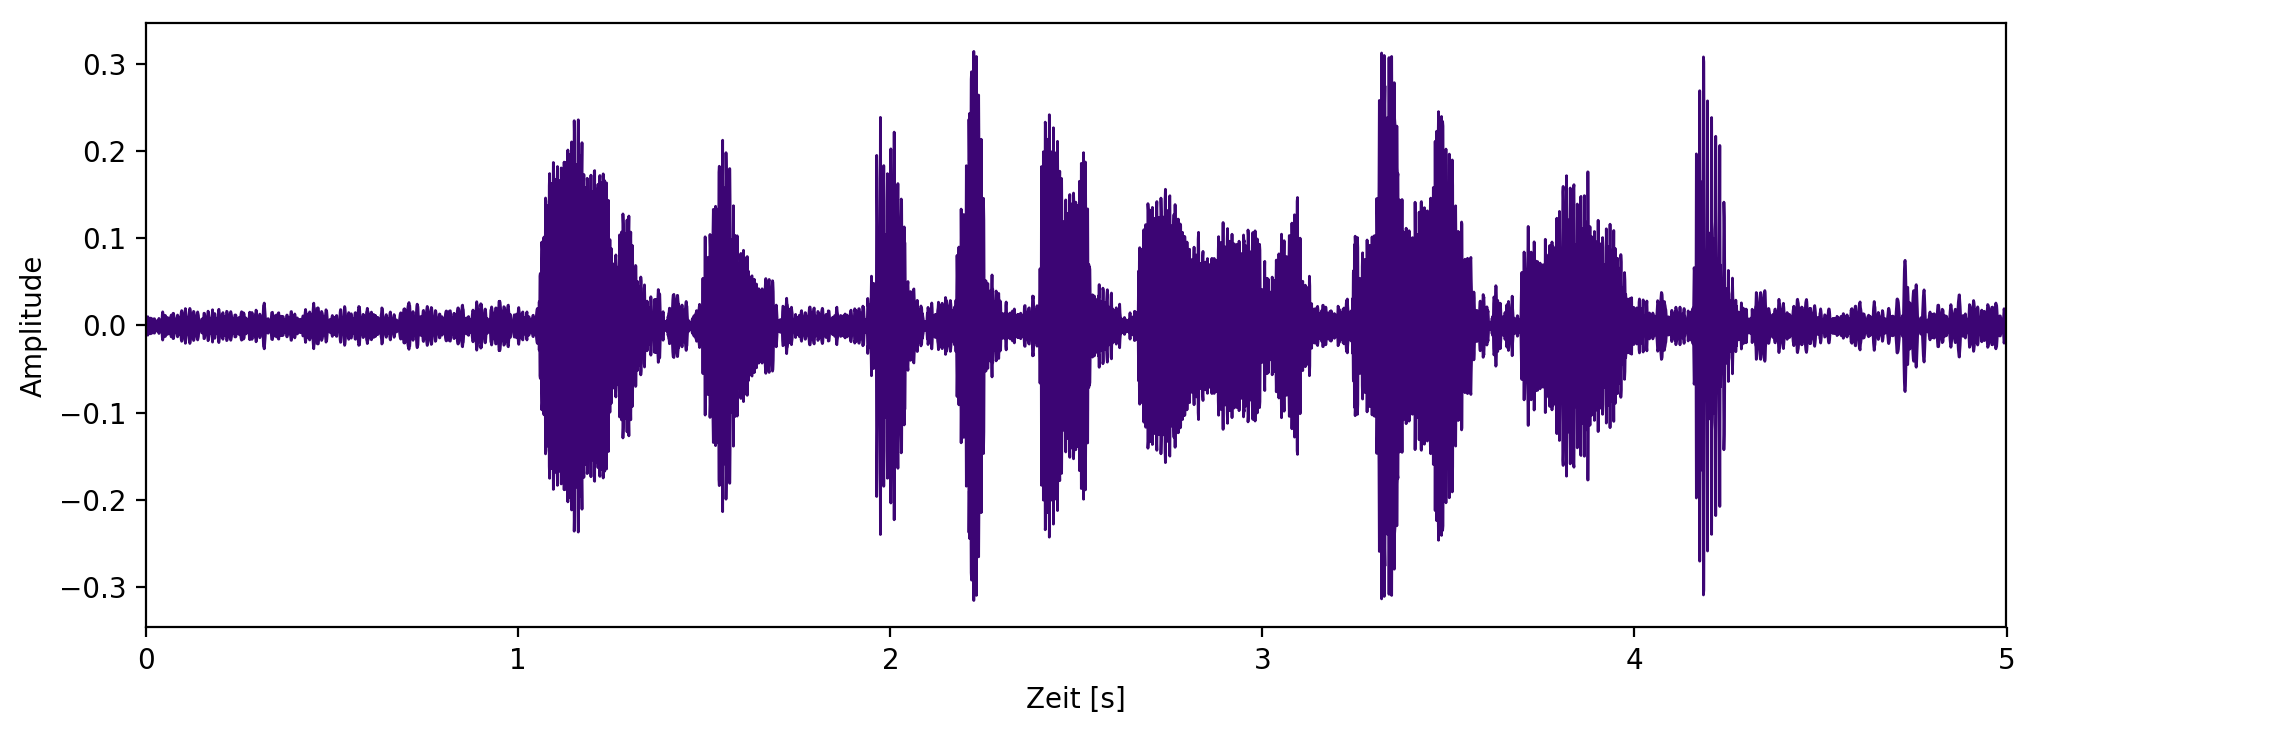
\includegraphics[width=0.6\textwidth]{assets/audio_raw.png}
		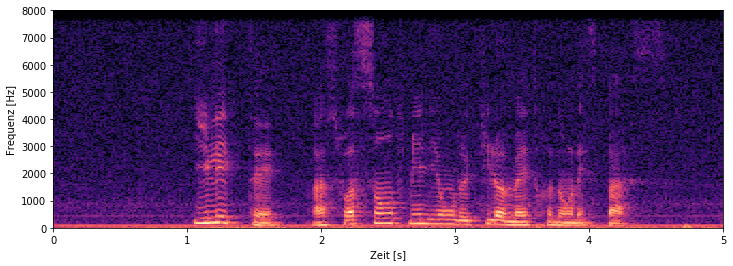
\includegraphics[width=0.6\textwidth]{assets/audio_log.png}
		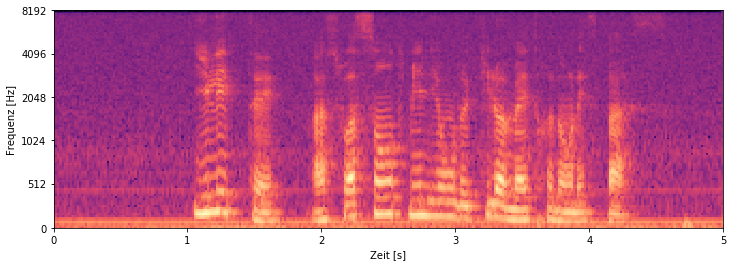
\includegraphics[width=0.6\textwidth]{assets/audio_mel.png}
	\centering
	\caption{Audio-Preprocessing: \textit{(oben)} Rohe Schallwelle, \textit{(mitte)}
		     Dezibel-Spectrogramm, 
		     \textit{(unten)} Mel Dezibel-Spectrogramm}
	\label{img:preprocessing}
\end{figure}
Spektrogramme \index{Spektrogramme}sind grafische Darstellungen eines Hörsignals nach der Anwendung der Fourrier-Transformation\parencite[]['Spectrograms']{fourrier}, ersichtlich in Abbildung \ref{img:preprocessing} \textit{(Mitte)}. Frequenzen über 10kHz können abgeschnitten werden, da menschliche Sprache grösst Teils darunter abläuft\parencite{tenkHz}. Im Spektrogramm lassen sich von Auge Muster erkennen und unterscheiden. Der visuelle Charakter der Spektrogramme erlaubt ausserdem das verwenden von \textit{Convolutional Neural Networks}.

\subsubsection{Mel Filtering}

Spektrogramme haben relativ viele Datenpunkte und sind deshalb recht aufwändig zu verarbeiten. Ein weiter \textit{preprocessing} Schritt wird deshalb oft angewendet: \textit{Mel Filtering}\parencite{mel}. Die Frequenzen werden dabei in grössere Eimer gepackt. Unter 1kHz sind die Eimer linear verteilt und darüber logarithmisch, siehe Abbildung \ref{img:preprocessing} \textit{(unten)}. Das Modell entspricht unserer Hörfähigkeit, die recht präzise unter 1kHz arbeitet, höhere Frequenzen aber schlecht unterscheiden kann\parencite{tenkHz}. 

\subsubsection{Implementation}

Die Oben genannten Transformationen können vor dem Training direkt auf die Daten angewendet und abgespeichert werden. In diesem Fall hätte man die rohen Daten löschen können. Allerdings sollte in dieser Arbeit sowohl an den rohen Daten wie auch an der Transformation flexibel experimentiert werden können, weswegen die Daten unbedingt beibehalten werden mussten. 

Anstatt die Transformationen selber zu implementieren wird ein Framework verwendet. In diesem Fall bietet sich an \textit{kapre}\parencite{kapre} an. Mit Kapre lassen sich währende dem Training die Daten in Echtzeit verarbeiten. Das Training dauert dabei aber 20\% länger. Konkret verhält sich \textit{kapre} wie eine Schicht vor dem eigentlichen Neuronalen Netzwerk.
\begin{figure}[hbt]
	\centering
		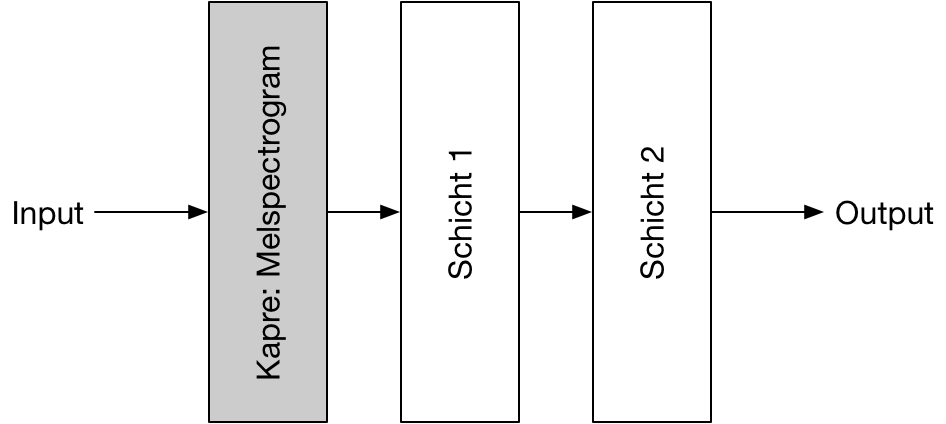
\includegraphics[width=0.6\textwidth]{assets/kapre.png}
	\centering
	\caption{\textit{Kapre}\parencite{kapre} als Schicht}
	\label{img:kapre}
\end{figure}


	          \section{Modelle}
Im folgenden Teil werden die entwickelten Deep Learning Modelle vorgestellt. Für jedes Modell ist der grundlegende Ablauf derselbe (siehe Abbildung \ref{img:workflow}). Die Aufnahme wird vorab auf die Länge 5s zugeschnitten. Anschliessend wird ein Spektrogramm generiert. Die Werte des Spektrogramms werden in die Dezibell Skala umgerechnet und dann normiert. Die Grösse des Spektrogramms unterscheidet sich zwischen den Modellen. Schliesslich berechnet ein Neuronales Netzwerk aus dem Spektogramm eine Vorhersage für die drei Sprachen. 
\\
Insgesamt werden drei grundsätzlich verschiedene Neuronalen Netzwerk Architekturen vorgestellt. Die ersten zwei Modelle sind Convolutional Neural Networks während das dritte Modell eine Kombination zwischen CNN und Recurrent Neural Network ist. Jedes Modell endet mit einer Ausgabeschicht der Grösse drei. Jeder der der drei Werte steht für die Wahrscheinlichkeit einer Sprache. Um zu garantieren, dass die Summe der Werte 1 gibt wird die Aktivierungsfunktion \textit{softmax} verwendet:
$$ \text{softmax}(\boldsymbol x)_i = \frac{\text{exp}(x_i)}{\sum_{j=0}^{n} \text{exp}(x_j)}$$
Beispiel: 
$$ \text{softmax}(\begin{bmatrix} 0.5 & 0.8 & 0.3\end{bmatrix}) = \begin{bmatrix} 0.31 & 0.43 & 0.26\end{bmatrix} = \begin{bmatrix} p_{FR} & p_{EN} & p_{DE}\end{bmatrix}$$
Die Funktion eignet sich generell für Klassifizierung, denn sie bildet die Werte auf eine Wahrscheinlichkeitsverteilung über die berechneten Ausgabeklassen ab \parencite[][S. 180-184]{goodfellow}. Der Wert einer Ausgabeklasse lässt sich auf diese Weise als die Wahrscheinlichkeit $p_{X}$ interpretieren: Die Wahrscheinlichkeit, dass die Eingabe in der Sprache X ist. Für alle anderen Schichten wird immer die Aktivierungsfunktion \textit{ReLU} verwendet.
\\
Damit die Ziele des Netzwerks die gleichen Anzahl Dimensionen wie die Ausgaben haben, werden sie \textit{One-hot}\parencite{chollet} kodiert. Das bedeutet, dass die richtige Sprache die Wahrscheinlichkeit 1.0 besitzt und alle anderen 0. Das Ziel für eine französische Aufnahme ist also $\begin{bmatrix} 1.0 & 0.0 & 0.0\end{bmatrix}$, für eine englische Aufnahme $\begin{bmatrix} 0.0 & 1.0 & 0.0\end{bmatrix}$, etc.. Obwohl die Ziele die gleiche Form wie die Ausgaben haben lässt sich der Verlustwert nicht so leicht berechnen wie beim Anfangsbeispiel. Die standard Verlustfunktion in diesem Fall ist \textit{Categorical Crossentropy}\parencite{chollet}. Für das Ziel $\boldsymbol{p} \in \mathbb{R}^n$ und die Voraussage $\boldsymbol{\hat{p}} \in \mathbb{R}^n$ ist die Funktion folgendermassen definiert:

$$H(\boldsymbol{p}, \hat{\boldsymbol{p}}) = -\sum\limits_{i} p_i \cdot \log \hat{p_i}$$
\\
Dass diese Verlustfunktion sinnvoll ist, lässt sich intuitiv verstehen: Das Ziel des Netzes soll es sein, die Wahrscheinlichkeit der richtigen Sprache zu maximieren. So soll zum Beispiel bei $\boldsymbol{p}=\begin{bmatrix} 0 & 1.0 & 0\end{bmatrix}$ und $\boldsymbol{\hat{p}}=\begin{bmatrix} p_0 & p_1 & p_2\end{bmatrix}$,  $ p_1$ maximiert werden. Die Wahrscheinlichkeit der richtigen Sprache lässt sich einfach berechnen:
$$L(\boldsymbol{p}, \hat{\boldsymbol{p}}) = \sum\limits_{i} p_i \cdot \hat{p_i}$$
Im Beispiel oben fallen $P_0$ und $P_2$ weg und $1\cdot P_1$ bleibt übrig, was genau der Wahrscheinlichkeit der richtigen Sprache entspricht. Ab hier lässt sich nachvollziehen, das genau wie wir $L$ maximieren wollen, $-L$ (wie der Verlustwert) minimiert werden soll. Da $\text{log}$ eine monoton steigende Funktion ist, ist $f(x)$ an der gleichen Stelle minimal wie $f(\log x)$. Was folgt ist genau die Categorical Crossentropy. Kurzgesagt sind die Parameter des Netzwerk die selben wenn $H$ minimiert oder $L$ maximiert wird: \parencite[vgl. ][]{entropy}
\begin{align*}
\shortintertext{Sei $X\in \mathbb{R}^n$ alle Parameter des Netzwerks so dass}
   L(\boldsymbol{p}(X), \boldsymbol{\hat{p}}) &= \max\limits_x\{L(\boldsymbol{p}(x), \boldsymbol{\hat{p}})\}
\shortintertext{folgt, dass}
-L(\boldsymbol{p}(X), \boldsymbol{\hat{p}}) &= \min\limits_x\{-L(\boldsymbol{p}(x), \boldsymbol{\hat{p}})\}
\shortintertext{und daraus folgt, dass}
-L(\boldsymbol{p}(X), \log\boldsymbol{\hat{p}}) &= \min\limits_x\{-L(\boldsymbol{p}(x), \log\boldsymbol{\hat{p}})\}\\
H(\boldsymbol{p}(X), \boldsymbol{\hat{p}}) &= \min\limits_x\{H(\boldsymbol{p}(x), \boldsymbol{\hat{p}})\}
\end{align*} 


Die Hyperparameter der Modelle, wie zum Beispiel die Grösse des Spektrogramms wurden empirisch bestimmt. Insgesamt wurden fast 200 Experimente durchgeführt. Allerdings konnte längst nicht jede mögliche Kombination von Hyperparametern probiert werden, da jeder Durchlauf zeitaufwändig und nicht parallelisierbar ist.
\begin{figure}[hbt]
	\centering
		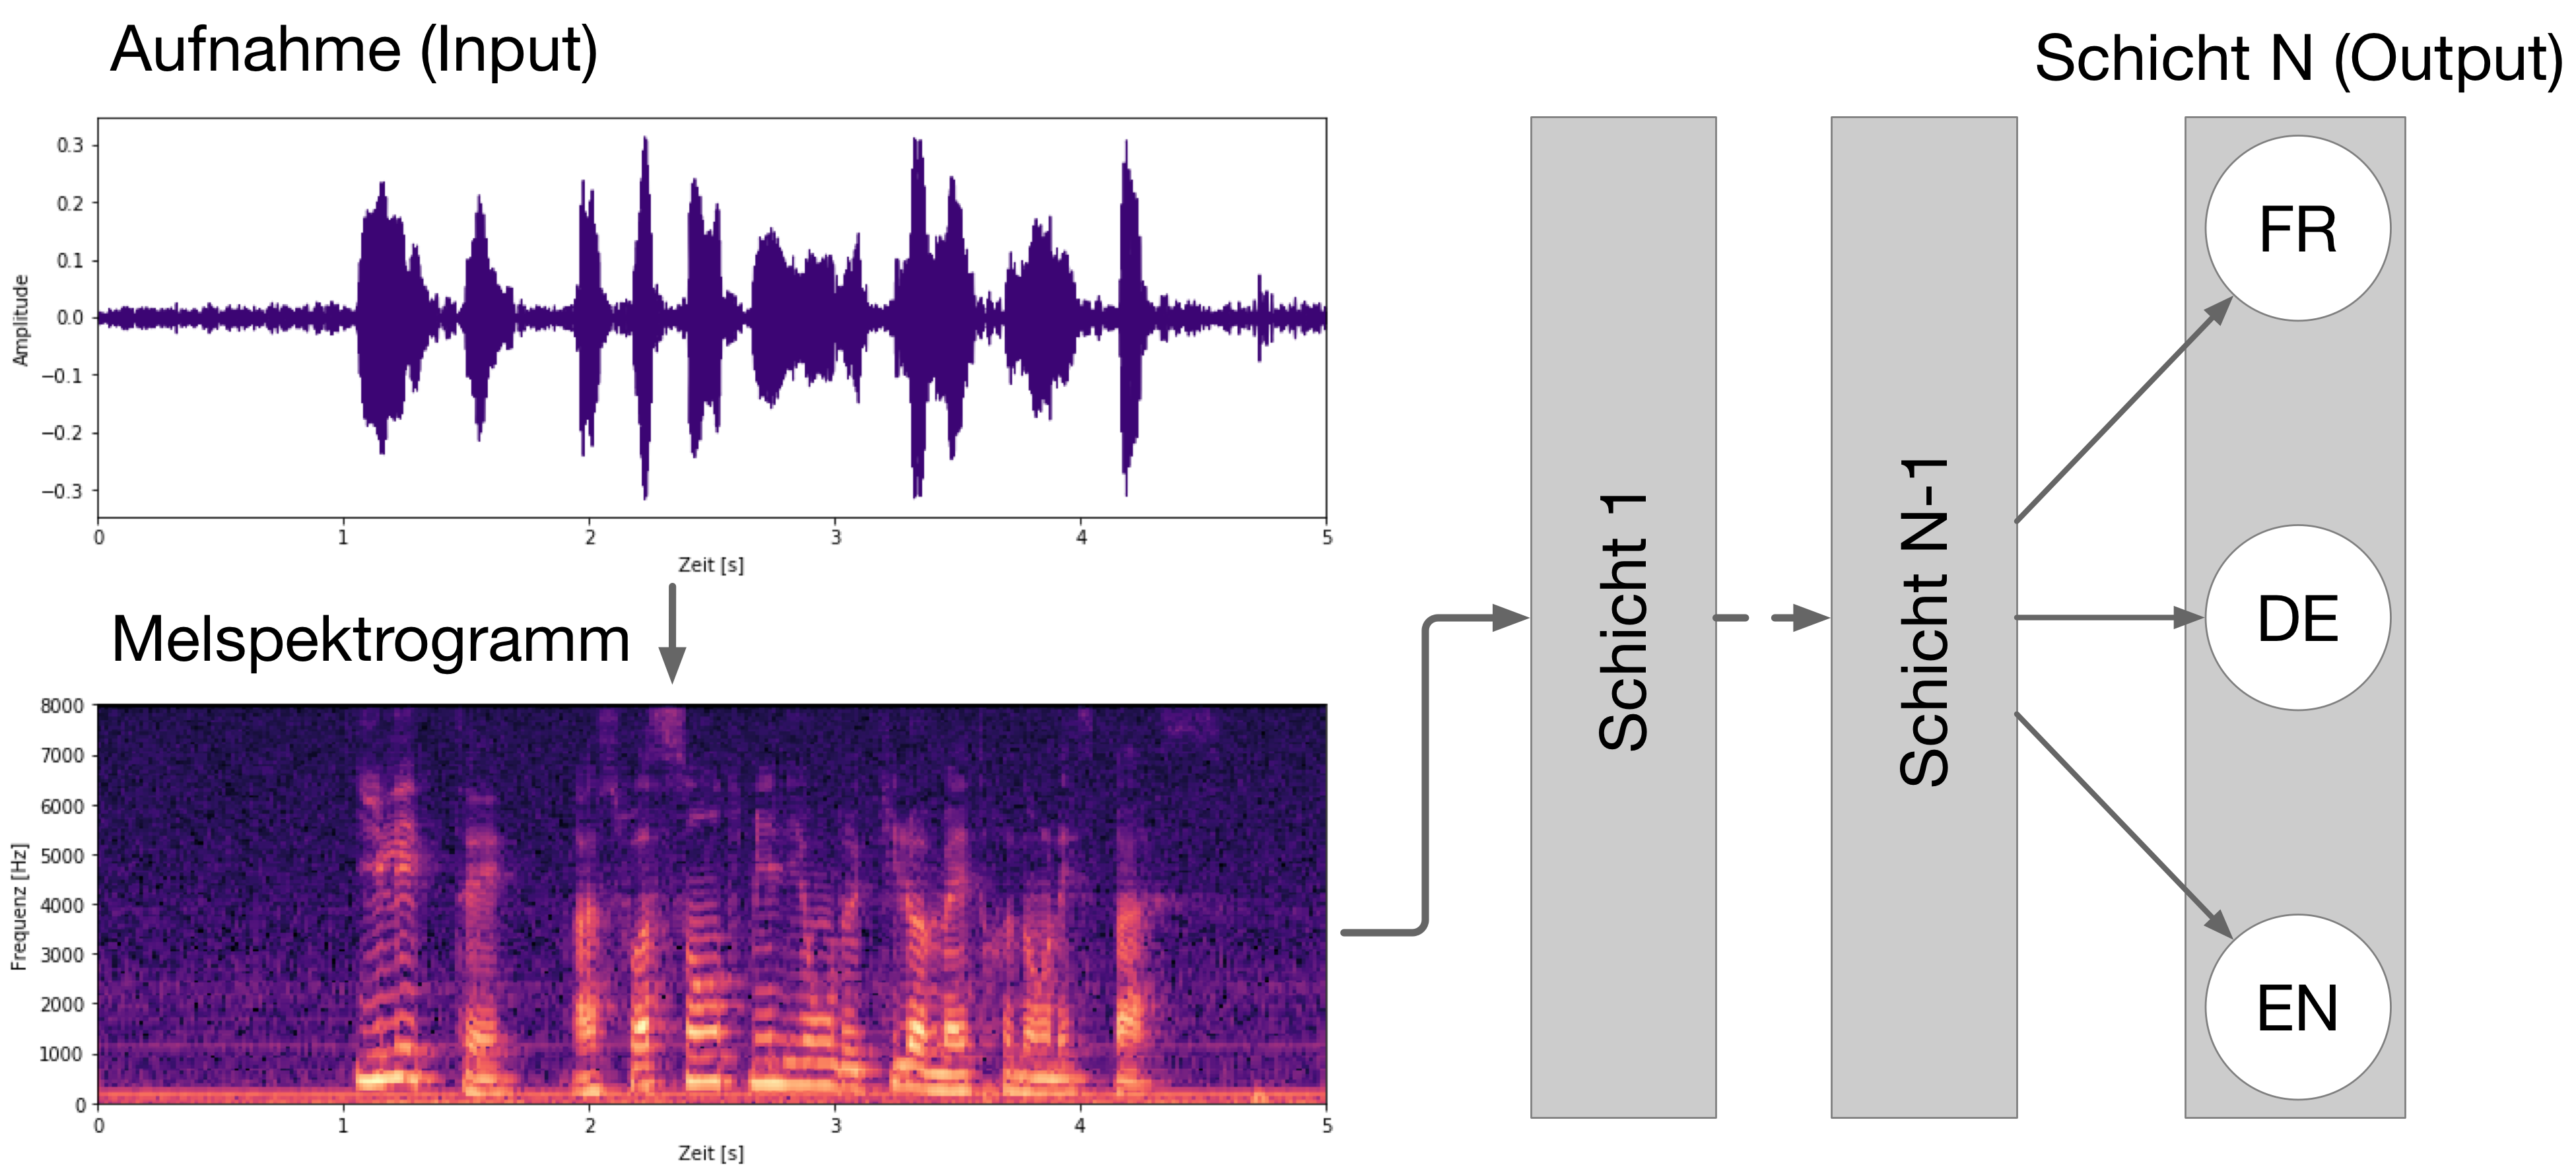
\includegraphics[width=0.8\textwidth]{assets/modelflow.png}
	\caption{Grundlegender Aufbau aller Modelle}
	\label{img:workflow}
\end{figure}


\subsection{CNN}
Das CNN Netzwerk akzeptiert Spektrogramme der Grösse 28x313, wobei 28 verschiedene Mel-Frequenzeimer berechnet werden an 313 Zeitpunkten. Das Netz besteht aus drei Convolution-MaxPooling Blocks und zwei Dense Schichten (Abbildung \ref{img:cnn}). Die Convolution-Grösse ist immer 3x3 und MaxPooling geschieht im Bereich 2x2. Die Anzahl Convolution's (Kanäle) nimmt von 64 auf 128 zu. 
\\
Die \textit{Fully Connected} Schicht besteht aus 512 Knoten mit 30\% \textit{Dropout}. Bei Dropout wird ein zufälliger gewählter Anteil der Eingabe der Schicht mit 0 ersetzt. Das Netz lernt dann, ohne diese Verbindungen auszukommen und somit mehrere Verbindungen einzelnen starken Verbindungen vorzuziehen. Die Eigenschaft hat einen positiven Einfluss auf die Robustheit des Netzes gegenüber neuen Daten \parencite[][Kap. 4.4.3]{chollet}.
\\
Die Architektur entspricht massgeblich der vorgestellten Architektur in \parencite{iLID} plus Dropout.
 \begin{figure}[hbt]
	\centering
		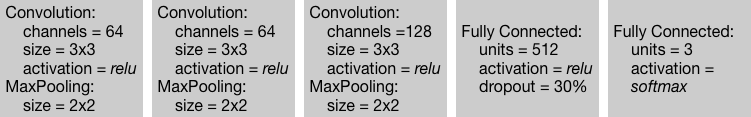
\includegraphics[width=0.8\textwidth]{assets/cnn.png}
	\caption{CNN Architektur}
	\label{img:cnn}
\end{figure}

\subsection{MobileNet-CNN}
Andere Arbeiten hatten gezeigt, dass grosse CNN Architekturen die auf dem \textit{ImageNet}\parencite{imagenet} Datenset (Riesiges Bilddatenset mit tausenden Bidklassen) stark sind, ebenfalls für Audioklassifizierung geignet sind \parencite{cnn_large}. Um Leistung zu sparen wurden Experimente mit \textit{MobileNet} durchgeführt.
MobileNet ist eine bekannte CNN Architektur entwickelt von \textit{Google} \parencite[][(V2)]{mobilenet}. Das Modell ist speziell entwickelt für Mobilgeräte, die in der Regel schwächere Hardware als Desktop-Computer besitzen. Das Ziel war ein effizientes Netzwerk für Bilderkennung im grossen Umfang, wie z.B ImageNet. Da das Modell in dieser Arbeit nur zwischen drei Klassen unterscheiden muss, wird die Anzahl Knoten im Netzwerk so weit wie möglich verkleinert, bzw. der Parameter $\alpha$ im Paper wird auf 0.25 gesetzt. 
\\
Das Netzwerk besitzt insgesamt 21 Schichten. Das Netzt funktioniert am bessten mit Eingaben der Grösse 224x224, der Bildgrösse in ImageNet. Die Spektrogramme werden darum auf dieses Format skaliert.
 \begin{figure}[hbt]
	\centering
		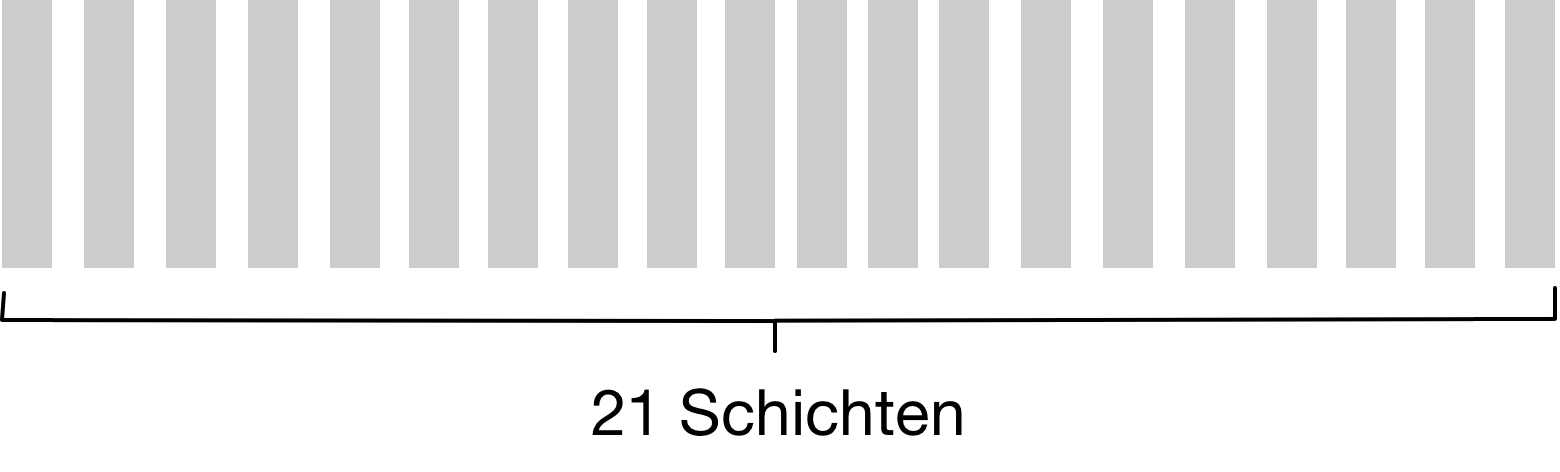
\includegraphics[width=0.8\textwidth]{assets/mobilenet.png}
	\caption{MobileNet Architektur}
	\label{img:mobilenet}
\end{figure}

\subsection{CRNN}
Convolutional Recurrent Neural Networks, eine Mischung aus CNN und RNN, wurden bereits erfolgreich auf Sprachidentifikation angewendet \parencite{crnn}\parencite{yerevann}. RNN's für Tonaufnahmen zu verwenden ist sinnvoll, denn Audiodaten sind naturgemäss zeitliche Folgen, also ideal für RNN's. RNN's haben aber den Nachteil, dass sie langsam lernen. Darum soll der CNN Teil im Vorfeld aus dem Spektrogramm eine kompaktere Repräsentation berechnet, z.b eine Abfolge von Phonemen. Da die Lernzeit proportional zur Eingabegrösse ist, lernt der RNN teil mit dieser Eingabe schneller. Es gibt keine Möglichkeit zu verifizieren, ob das CNN wirklich Phoneme berechnet aber die Resultate zeigen, dass das CRNN besser abschneidet als das CNN.
\\
Der CNN Teil besteht aus fünf Blocks von Convolution, MaxPooling und \textit{Batch Normalization}\label{Batch Normalization} (Siehe Abbildung \ref{img:crnn}). Die Idee von \textit{Batch Normalization} ist, dass die Ausgabe der vorherigen Schicht so normalisiert wird, dass sie den Durchschnitt 0 und die Varianz 1 besitzt. \textit{Batch Normalization} bringt den vor allem den Vorteil, dass das Modell schneller konvergiert, also schneller bessere Leistungen erbringt. \parencite{batch}
\\
Die Anzahl Convolutions steigert sich schrittweise von 16 auf 64. Das Convolution-Fenster hat immer die Grösse 4x4 und MaxPooling das Fenster 2x2. Bei den Convolutions wird 0.01 \textit{L2-Regularisation} verwendet:
$$ Verlust = Verlust + \sum_{i} w_{i}^{2}$$
Das bedeutet, dass dem Verlustwert zusätzlich das Quadrat der Gewichte addiert wird \parencite[Kap.~7.1.1]{goodfellow}. Übermässig hohe Gewichte werden überproportial gewertet. Die Regularisation hat das gleiche Ziel wie Dropout, das Netz robuster zu gestalten.
\\

 \begin{figure}[hbt]
	\centering
		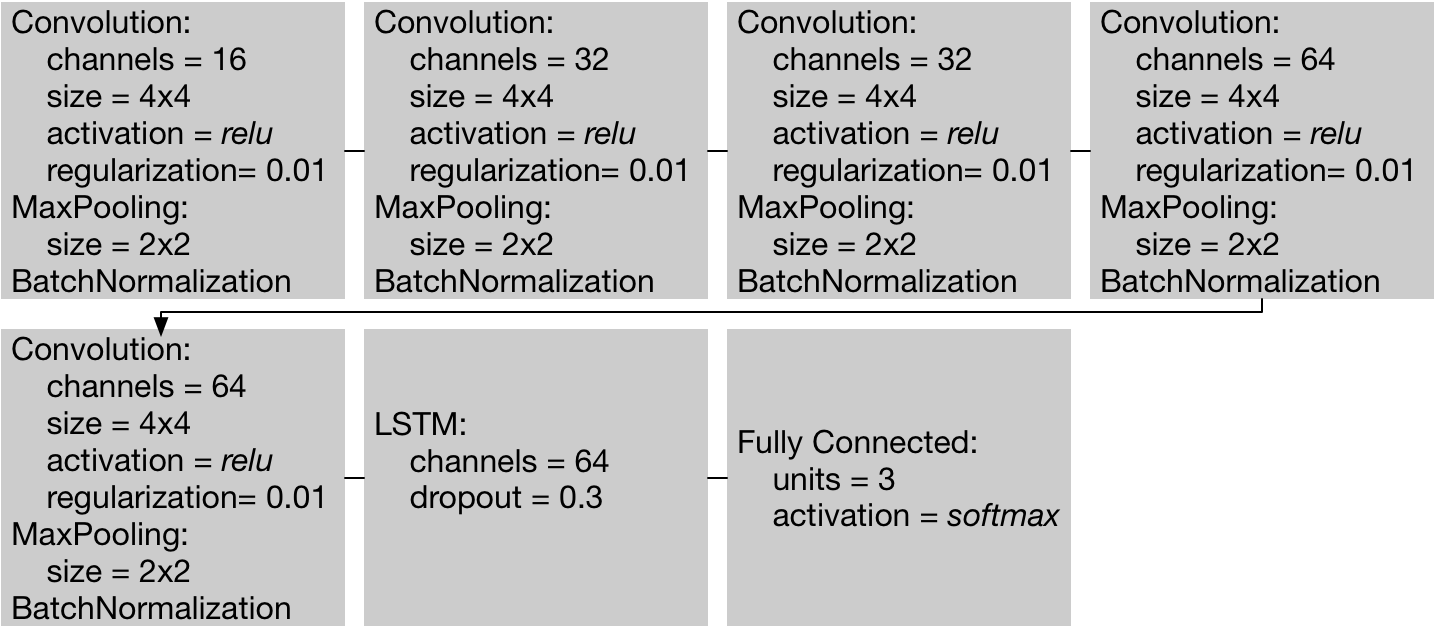
\includegraphics[width=0.8\textwidth]{assets/crnn.png}
	\caption{CRNN Architektur}
	\label{img:crnn}
\end{figure}

\section{Umsetzung und Resultate}

\subsection{Implementierung}

Was in dieser Arbeit theoretisch gemacht wurde, wurde bis hierhin ausführlich beschrieben. Die praktische Implementierung aller Schritte wurde aber noch nicht behandelt. Dieses Kapitel erklärt die genaue Umsetzung aller Teile und nennt die verwendeten Werkzeuge. In anderen Worten wird hier die praktische Arbeit anschaulich gemacht.
Für alle Teile der Arbeit wird mir der Programmiersprache \textit{Python}  gearbeitet. Python eignet sich generell für Deep Learning weil viele Bibliotheken für die Sprache geschrieben sind. Ausserdem hat Python den Vorteil, dass es einsteigerfreundlich ist. Python kann entweder als Script geschrieben werden, also als Datei die ausgeführt wird, oder in einem interaktiven \textit{Jupyter Notebook}\parencite{jupyter}. Jupyter Notebook's  bestehen unter anderem aus mehreren Textzellen die einzeln ausgeführt werden können aber den gleichen Thread teilen. Das macht Jupyter Notebooks unglaublich praktisch für das Experimentieren und Darstellen von Daten.
\\ \\
Die Aufgabe lässt sich in vier Teile gliedern. Abbildung \ref{img:vorgehen} zeigt die Teile schematisch. 
Als erstes müssen die zu verwendeten Daten aus den verschiedenen Quellen gesammelt werden. Bevor die Daten aber heruntergeladen werden muss in manchen Fällen eine Selektion geschehen. So kann bei Youtube aufgrund der riesigen Anzahl an verfügbaren Videos unmöglich die gesamte Datenmenge gesammelt werden. Aus diesem Grund wurde bei Youtube manuell nach geeigneten Kanälen bzw. Playlists gesucht. Nach dem klar ist was gesammelt werden soll kann man mit dem Herunterladen starten. Dafür werden Python-Scripts geschrieben die die beträchtliche Menge Daten automatisiert herunterladen. Für die YouTube Daten wird die externe Bibliothek \textit{Youtube-dl}\parencite{youtube-dl} benutzt.

 \begin{figure}[hbt]
	\centering
		
\includegraphics[width=1.0\textwidth]{assets/vorgang_small.png}
	\caption{Überblick über die Arbeitsschritte}
	\label{img:vorgehen}
\end{figure}

Der zweite Schritt ist das Erforschen der Daten. Darunter wird zum Beispiel das herausarbeiten von wichtigen Unterschieden zwischen den Datenquellen verstanden. Unter anderem wurde in diesem Schritt eine einheitliche Länge und Abtastrate der Aufnahmen festgelegt. Für diesen Teil sind Jupyter Notebook's ideal.  Für das einlesen der Audiodaten wird die Bibliothek \textit{Librosa}\parencite{librosa} verwendet und alfällige Grafiken werden mit der Bibliothek \textit{Matplotlib}\parencite{matplotlib} erstellt.
\\
Als nächstes können die Daten korrekt strukturiert werden. Das heisst das die Daten einerseits in Training, Validation und Testdaten gespalten werden während sie gleichzeitig nach der Sprache geordnet sind. Vor dem definitiven abspeichern der Daten werden sie auch auf die richtige Länge zugeschnitten. Das Format der Daten ist ein \textit{Numpy}-Array\parencite{numpy}. Numpy stellt praktische Funktionen für numerische Operationen bereit und kann die Daten effizient abspeichern. Programmiert wird dieser Teil in einer Mischung aus Python-Scripts und Jupyter Notebook's.
\\
Zum Schluss kommt Machine Learning ins Spiel. Der letze Schritt ist das Experimentieren mit unterschiedlichen Modellen. Erst jetzt werden Netzwerke trainiert und ausgewertet. Die zwei wichtigen Bibliotheken für den Machine Learning Teil sind \textit{Keras}\parencite{keras} und \textit{Tensorflow}\parencite{tensorflow}. Tensorflow ist die Machine Learning Bibliothek von Google. Dank Tensorflow müssen keine neuronalen Netze von Grund auf programmiert werden. Tensorflow übernimmt alle Arbeit ausser das tunen von Hyperparametern. Keras ist lediglich ein einfaches Interface für Tensorflow und andere Machine Learning Bibliotheken. Der Code für das Trainieren eines einfachen Keras Modells findet sich im Anhang. 


\subsection{Auswertung an Voxforge und YouTube}

An dieser Stelle werden die drei Modelle ausgewertet. Es wird gemessen wie gut die Modelle Aufnahmen klassifizieren. Die verwendete Messgrösse um die Modelle zu vergleichen ist die Genauigkeit. Die Genauigkeit beschreibt den Anteil an richtig klassifizierten Aufnahmen:
$$Genauigkeit = \frac{\# \text{ Korrekt klassifizierte Aufnahmen}}{\# \text{ Total Aufnahmen}}$$
Genauigkeit ist in diesem Fall eine angebrachte Messgrösse, weil die Daten gleichmässig über die Sprachen verteilt sind. Ist dies nicht der Fall kann die Genauigkeit täuschen. Wenn zum Beispiel 90\% der Daten Deutsch wären, würde hypothetisch ein Modell dass immer Deutsch ausgiebt 90\% Genauigkeit haben. Obwohl das hypothetische Modell extrem naiv ist, täuscht die hohe Genauigkeit. Im Fall dieser Arbeit wurde darum ausdrücklich auf eine gleichmässige Verteilung der Daten geachtet.
\\ 
Die Modelle werden separat an allen drei Datenquellen ausgewertet. Für jedes Datenset wurden alle Modelle drei Mal trainiert. Die schlussendliche Genauigkeit ist die beste der drei Versuchen. Die Genauigkeiten am Voxforge Testset sind in Tabelle \ref{table:test_vox} geschrieben.
\begin{table}[h]
	\centering
	\begin{tabular}{llll}
		\hline
		Netz & Architektur     & Genauigkeit \\ \hline
		CNN  & 3 Conv          & 95.5\%      \\
		CRNN & 4 Conv + GRU   & 96.9\%       \\
		MobileNet  & 28 Conv + Dense & 86.1\%       \\ \hline
	\end{tabular} \\
	\caption{Beste Voxforge Genauigkeit}
	\label{table:test_vox}
\end{table}
Das CRNN führt mit fast 97\%, dicht gefolgt vom CNN. Das MobileNet besitzt eine mehr als 10\% tiefere Genauigkeit. Obwohl der Unterschied zwischen CRNN und CNN absolut klein erscheint, ist er relativ zum Fehler beträchtlich. Das CRNN hat eine mehr als 30\% kleinere Fehlgenauigkeit als das CNN.
\\ 
Die Genauigkeiten am Youtube Testset zeigt Tabelle \ref{table:test_you}. Sämtliche Modelle haben am Youtube Testset eine tiefere Genauigkeit als am Voxforge Testset. Das MobileNet vollzieht mit einem Verlust von 5.9\% Genauigkeit den grössten Fall. Das CNN und CRNN besitzen beide eine Genauigkeit von 94.7\%.
\\
Die bisherigen Resultate zeigen, dass das CRNN insgesamt die höchste Genauigkeit hat. Trotzdem heisst das nicht, dass das CRNN in jedem Fall besser ist als die anderen beiden Modelle. Der Beweis dafür ist, dass eine Kombination aller Modelle oft besser ist, als die einzelnen Modelle. Ein Modell berechnet aus dem Durchschnitt der drei Modelle erreicht bei Voxforge eine Genauigkeit von 97.9\%. Das bedeutet eine erneute Verkleinerung der Fehlgenauigkeit um mehr als 30\%.
\begin{table}[h]
	\centering
	\begin{tabular}{llll}
		\hline
		Netz & Architektur     & Genauigkeit  \\ \hline
		CNN  & 3 Conv          & 94.7\%       \\
		CRNN & 4 Conv + LSTM   & 94.7\%     \\
		MobileNet  & 28 Conv + Dense & 80.2\%   \\ \hline
	\end{tabular}
	\caption{Beste YouTube Genauigkeit}
	\label{table:test_you}
\end{table}
\\
Das CRNN hat die höchste einzelne Genauigkeit zum Preis einer langen Trainingsdauer. Das CRNN braucht mehr als drei mal so lang zum trainieren wie das CNN. Das Genauigkeit/Zeit Verhältnis des CNN ist bedeutend grösser als das des CRNN. Die Trainingszeiten sind in Tabelle \ref{table:test_time} aufgetragen.
\begin{table}[h]
	\centering
	\begin{tabular}{lll}
		\hline
		Netz & Trainingsdauer \\ \hline
		CNN  & 20 min \\
		CRNN & 70 min \\
		MobileNet  & 60 min\\ \hline
	\end{tabular}
	\caption{Trainingsdauer}
	\label{table:test_time}
\end{table}
\\
Eine weitere Methode um neben der Genauigkeit die Modelle auszuwerten, ist eine Wahrheitsmatrix aufzustellen. Die Zeilen der Matrix entsprechen der Sprache der Aufnahmen, während die Spalten die berechnete Antwort des Algorithmus unterscheiden. Das Feld oben links zeigt zum Beispiel die Anzahl der französischen Aufnahmen die als Französisch klassifiziert wurden. Die Wahrheitsmatrix gibt zeigt somit mehr Details als die Genauigkeit alleine. Abbildung \ref{img:matrix_vox} zeigt die Matrix vom CRNN Modell an den kombinierten Testdaten von Youtube und Voxforge.
\\
Das interessante das an dieser Matrix ablesbar ist, ist dass das Modell Englisch und Deutsch relativ oft verwechselt: Englisch wird in 121 Fällen mit Deutsch verwechselt und Deutsch wird 122 mal dem Englischen verwechselt. Im Vergleich werden Französisch und Deutsch insgesamt nur in 67 Fällen verwechselt. Französisch und Englisch werden insgesamt 105 mal verwechselt.
 \begin{figure}[hbt]
	\centering
		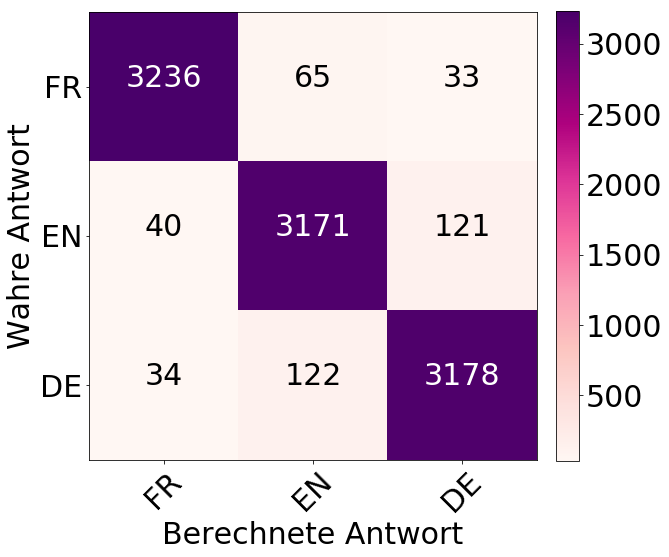
\includegraphics[width=0.5\textwidth]{assets/matrix_voxyou_crnn.png}
	\caption{Wahrheitsmatrix von CRNN an Voxforge und Youtube (Total 10'000 Aufnahmen)}
	\label{img:matrix_vox}
\end{figure}

\subsection{Auswertung an Librivox}
Die Genauigkeit bei den Voxforge und Youtube Daten war sehr hoch, weil die Modelle die beiden Quellen bereits kannten. Obwohl das Testset unterschiedlich vom Trainingsset ist,  teilen sie viele Gemeinsamkeiten. Die Librivox Daten sind den Modellen hingegen komplett fremd. Mit der Auswertung an den Librivox Daten wird klar, wie gut das Modell generalisiert, bzw. wie gross die Stichprobenverzerrung ist.
\\
Tabelle \ref{table:test_lib} zeigt die Genauigkeiten auf dem Librivox Testset. Das CNN verliert im Vergleich zu vorher rund 6\% Genauigkeit. Das CRNN hingegen erreicht immer noch 94.1\% Genauigkeit. Am schlimmsten geht es dem MobileNet, das auf eine Genauigkeit von 56.8\% sinkt. Anhand dieses Verlust lässt sich klar ablesen, dass das MobileNet sich an die Trainingsdaten überangepasst hat. Das CRNN und CNN auf der anderen Seite generalisieren überraschend gut.
\begin{table}[h]
	\centering
	\begin{tabular}{llll}
		\hline
		Netz & Architektur     & Genauigkeit  \\ \hline
		CNN  & 3 Conv          & 88.1\%       \\
		CRNN & 4 Conv + LSTM   & 94.1\%       \\
		MobileNet  & 28 Conv + Dense & 56.8\%       \\ \hline
	\end{tabular}
	\caption{Beste Librivox Genauigkeit}
	\label{table:test_lib}
\end{table}
\\
Genau wie bei Voxforge und Youtube lässt sich wieder eine Wahrheitsmatrix zu detaillierten Auswertung erstellen. Abbilung \ref{img:matrix_lib} zeigt die Matrix des CRNN Modells. Auffällig an dieser Matrix ist, dass Englisch relativ selten mit anderen Sprachen verwechselt wird. Deutsch und Französisch werden hingegen oft fälschlicherweise als Englisch erkannt. 
\begin{figure}[hbt]
	\centering
		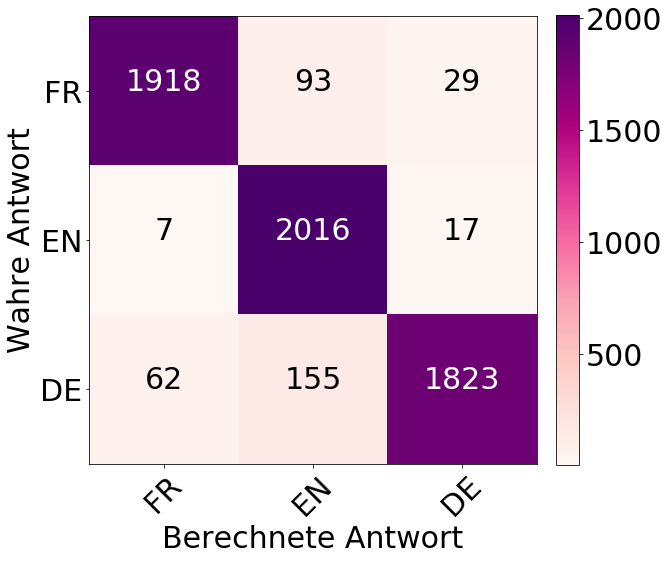
\includegraphics[width=0.5\textwidth]{assets/matrix_lib_crnn.png}
	\caption{Wahrheitsmatrix von CRNN an Librivox (Total 6120 Aufnahmen)}
	\label{img:matrix_lib}
\end{figure}

	\section{Diskussion}
Im Rahmen dieser Arbeit wurde ein System zum klassifizieren von Sprachaufnahmen implementiert. Das Programm unterscheidet zwischen Französisch, Deutsch, und Englisch. Mit Deep Learning hat das Programm selbst gelernt die Sprache von kurzen Aufnahmen zu erkennen. Anstatt rohe Schallwellen zu verarbeiten wurden in Echtzeit berechnete Spektrogramme verwendet. Die Spektrogramme konnten mit Bilderkennungsmethoden erfolgreich eingeordnet werden. Ein hybrides Modell aus CNN und RNN besass die höchste Genauigkeit. Die Trainingsdaten wurden wegen fehlenden maßgeschneiderten Datensets aus verschiednen Quellen selbst kompiliert. Es wurde mit Daten von Voxforge und Youtube trainiert um mit Daten aus der Librivox Hörbuchdatenbank getestet zu werden. Die hohe Korrektheit aller Modelle bestätigt, dass tiefe neuronale Netze eine angemessene Methode für Sprachidentifikation sind.
\\ \\
Der Vergleich der Resultate mit anderen Arbeiten ist nur mit Vorsicht möglich. Der wichtigste Unterschied ist, dass andere Daten verwendet werden und dementsprechend nur andere Resultate entstehen können. Glücklicherweise sind Arbeiten zu Automatischer Sprachidentifikation im Internet jedoch frei erhältlich, denn das Problem ist in der Informatik recht jung. Erst in den 70'er Jahren wurde man für das weiterleiten von Telefonanrufen auf das Thema aufmerksam. Eine lange Zeit galt, dass die bessten Systeme diejenigen waren, die die fortgeschrittensten sprachlichen Merkmale berechneten. Der Nachteil an diesen Systemen ist, dass die Erweiterung auf andere Sprachen mit einem grossem Aufwand verbunden ist. \parencite{history}
\\
Erst mit dem Aufkommen von Deep Learning als konkurrenzfähige Methode im letzen Jahrzehnt kamen wieder Systeme mit weniger Preprocessing auf \parencite{chollet}. 2009 erreichte Grégoire Montavon mit Deep Learning für 3 Sprachen auf dem Voxforge Datenset eine Genauigkeit von $80.1\%$ \parencite{montavon}. Das Voxforge Datenset hat sich seither verändert. Es kann angenommen werden, dass die hier vorgestellten Modelle, sein System deutlich übertreffen, da ähnliche Arbeiten dass getestet haben \parencite{iLID}. 2016 wurde mit einem sehr ähnlichen Modell wie das CNN Modell dieser Arbeit Genauigkeiten von 93\% und 85\% für 2 Sprachen respektive 4 Sprachen gemessen \parencite{iLID}. Hrayr et al. \parencite{yerevann} stellen im selben Jahr ein CRNN Modell für einen Wettbewerb vor, dass zwischen 176 Sprachen mit 99.67\% Genauigkeit differenzieren kann. Ein weiteres CRNN Modell von Bartz et al. \parencite{crnn} erreicht 2017 91\% bei der Unterscheidung von vier Sprachen.
\\
Die in dieser Arbeit vorgestellten System leisten vergleichbare Genaugigkeiten wie die genannten Modelle. 95\% ist eine höchst zufriedenstellende Genauigkeit unter anbetracht das das Youtube Datenset nicht fehlerfrei ist. Das Datenset wurde bekanntlich nicht manuell gesäubert. Es können dementsprechend Aufnahmen ohne Sprache oder mit fremdsprachigen Interviews enthalten sein. Der Anteil von fehlerhaften Aufnahmen ist jedoch wahrscheinlich klein. 
Der Fall auf 80\% Genauigkeit beim Librivox Datenset ist normal. Das Modell ist selbstverständlich für die Youtube und Voxforge Daten optimiert und nicht für Hörbücher. Die Librivox Daten haben zum Beispiel unterschiedliche Hintergrundgeräusche und Aufnahmeprotokolle. 80\% bleibt in jedem Fall ein erfreuliches Resultat. Ein Zufallsgenerator würde im Kontrast nur 33\% erreichen. Es kann also aus dem Resultat abgelesen werden, dass das Modell angemessen generalisiert. 
\\ \\
Bis jetzt wurde das Modell nur an öffentlich verfügbaren Daten ausgewertet wo klar war welche Sprache gesprochen wurde. In der Realität soll das Modell aber helfen die Sprache von unbekannten Aufnahmen zu erkennen. In anderen Worten soll das Modell in der Praxis angewendet werden. Dafür wurde ein Interface programmiert wo Benutzer sich selbst Aufnehmen und das Modell damit abfragen können. Das Interface ist in Form einer Webseite auf den Schulservern frei verfügbar. Die meisten Mobilgeräte und Computer sind kompatibel. Abbildung \ref{img:interface} zeigt die Seite nach dem hochladen einer zufälligen Aufnahme.
\begin{figure}[hbt]
	\centering
		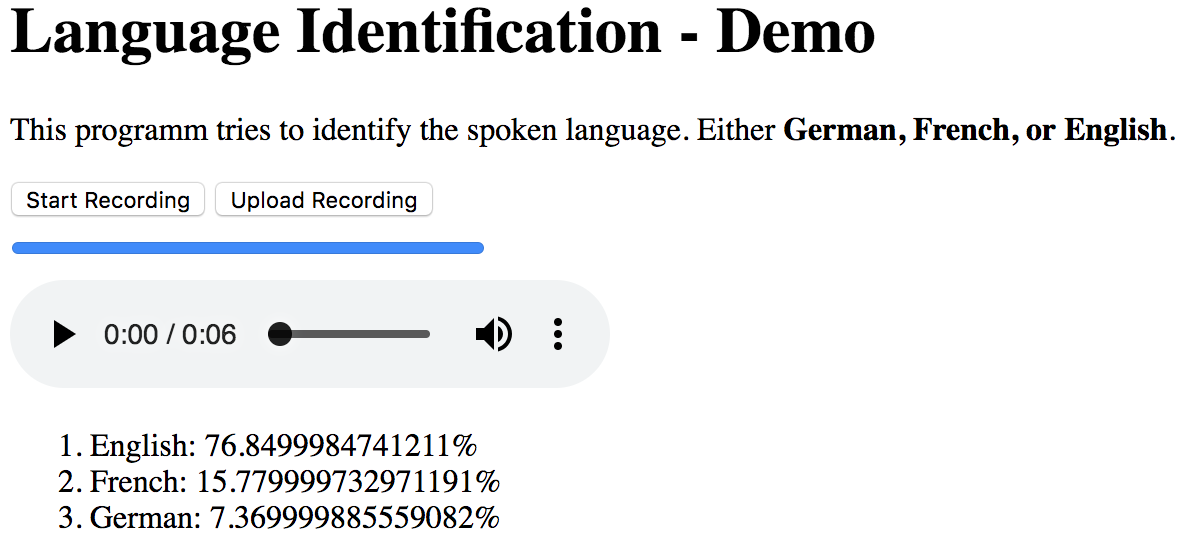
\includegraphics[width=0.6\textwidth]{assets/interface.png}
	\caption{Interface Schnappschuss}
	\label{img:interface}
\end{figure}
Die Umgebung bei Smartphone Aufnahmen ist erneut eine andere wie die von Voxforge und YouTube. Die Genauigkeit die dort erreicht wird ist eine weitere Art die Generalisierbarkeit des Modells zu messen. Aus Neugier wurde ein sehr kleines Datenset aus Aufnahmen von Verwandten und Freunden zusammengestellt. Es wurde darauf geachtet, dass die Sprache deutlich verständlich ist. Insgesamt sind es nur 70 ungleichmässig verteilte Aufnahmen. Die Resultate daraus sind wegen der kleinen Anzahl und Varianz kaum signifikant. Das Programm entdeckt in 70\% der Fälle die richtige Sprache. 
Eine Programm mit Genauigkeit 70\% ist in mancher Hinsicht kein guter Klassifizierer. Kommerziell einsetzbar ist das System damit sicherlich nicht. Für ein Callcenter würde das bedeuten, dass fast jeder dritte Anruf dem falschen Mitarbeiter zugewiesen wird. Das ist aus Sicht der Kunden katastrophal. Also stellt sich die Frage woher der Fehler kommt, bzw. was man noch verbessern kann.
\\ \\
An erster Stelle sind die Daten ein Problem. Die Trainingsdaten sind nicht repräsentativ für alle möglichen Daten, unter anderem Handy-Aufnahmen. Um die Stichprobenverzerrung weiter zu minimieren muss man mehr Daten beschaffen. Die Daten sollten so vielfältig wie möglich sein. Es ist nutzlos unendlich viele Daten zu besitzen wenn die sie sich alle sehr ähnlich sind. Einzelne relevante Merkmale sind unter anderem das Geschlecht, die Stimmhöhe, Hintergrundgeräusche, die Qualität der Aufnahme und die Geschwindigkeit. Je mehr Kombination es gibt desto besser. 
\\
Was macht man aber, wenn man nur eine begrenzte Menge an Daten zur Verfügung hat? In diesem Fall gibt es eine Methode namens \textit{Data Augmentation}. Die Lösung ist, aus den vorhanden Daten weitere Daten zu erschaffen. Manche Merkmale lassen sich nämlich automatisch anpassen. Beispielsweise kann der Computer ohne Problem die Geschwindigkeit und die Qualität der Aufnahme adaptieren. Der Computer passt bei Data Augmentation in jedem Durchlauf zufällig die Merkmale der einzelnen Aufnahmen an. Im Endeffekt wird dem Netzwerk also nie genau die gleiche Aufnahme gezeigt. Das verhindert das das Netzwerk sich an eine endliche Menge von Daten überanpasst. Zudem wird die Stichprobenverzerrung dadurch minimiert. In der Regel hat Data Augmentation immer einen positiven Effekt. Darum ist Data Augmentation  eine mächtige und weit verbreitete Methode.  In dieser Arbeit wurde primär keine Data Augmentation angewendet, weil man die falsche Vorstellung hatte, dass sowieso genug Daten vorhanden wären. Es stellt sich aber im Nachhinein heraus, dass Data Augmentation immer besser ist als dem Netzwerk die gleichen Daten mehrmals zu zeigen. 
\\
An zweiter Stelle sind Mängel beim Training. Die Abbildung mit dem Lernprozess zeigt wie uneben die Kurve der Validation Genauigkeit ist. Manchmal sinkt die Genauigkeit abrupt um im nächsten Durchlauf wieder zu steigen. Die Schwankungen können nur daran liegen, dass das Validationset und das Testset zu klein sind. Das führt dazu, dass sie leicht beeinflussbar sind. Eine Erhöhung auf 25\% der gesamten Daten ist für beide zu empfehlen. Andere Hyperparamter oder ganz andere Modelle könnten ebenfalls besser sein. Allerdings wird für viele Experimente ein leistungsstarker Computer benötigt. Mehr Leistung ist immer hilfreich.
\\
Noch mehr Verbesserungspotenzial liegt wahrscheinlich im Verfahren \textit{Learning from Between-class Examples for Deep Sound Recognition}(2017)\parencite{between}. Yuji et al. stellen eine vielversprechende Methode vor, die die Genauigkeit in jedem ihrer Versuche verbessert. Die Idee ist es, Aufnahmen von verschiedenen Klassen zu kombinieren um eine Mischaufnahme zu erfinden deren Ziel ebenfalls zwischen den Klassen liegt. Vereinfacht angewendet auf Sprachidentifikation könnte das bedeuten, dass eine deutsche und eine französische Aufnahme gleichzeitig abgespielt werden um zu einer Aufnahme kombiniert zu werden. In dieser Aufnahme würden also zwei Sprecher parallel sprechen. Das Ziel der Aufnahme wäre ebenfalls ein Mix z.B $\begin{bmatrix}0.5 & 0 & 0.5 \end{bmatrix}$. Das schöne am Verfahren ist, dass es einfach zu verstehen ist und doch sehr wirksam. Leider reichte die Zeit nicht aus um die Methode zu implementieren.
\\ \\ 
Egal wie viel Potential nach oben am Schluss noch bleibt, war die Arbeit ein Erfolg. Ausser dem Produkt ist immer auch der Weg das Ziel. Es wurde enorm viel gelernt und Erfahrung gesammelt über Deep Learning. Auf der einen Seite zeigt das Projekt wie erstaunlich einfach künstliche Intelligenz in der Praxis ist. Ohne jahrelanges Studium ist man in der Lage das meisste zu verstehen und zu implementieren. Nichts daran ist magisch. In vielerlei Hinsicht ist Deep Learning momentan keine absolute Wissenschaft mit wahr und falsch. Ein grosser Teil der Optimierung besteht aus heuristischen Experimenten. Bei Hyperparametern gibt es noch grossen Forschungsbedarf. Wenn einmal klar ist wie diese gesetzt werden müssen, wird Deep Learning wirklich bereit sein für jedermann. In Zukunft wird es wohl einfachere Inferfaces geben, denen man nur das Problem angeben muss und der Rest automatisch erledigt wird. Auf der anderen Seite ist Deep Learning mathematisch ein kompliziertes Gebiet. Die Grundlagen können in Zukunft nur noch anspruchsvoller werden. Wer wirklich mitforschen will, muss sehr stark in Mathematik sein. Lineare Algebra findet hier tatsächlich Anwendung. Ein ebenfalls nicht zu unterschätzender Teil war das Sammeln und Vorbereiten der Daten. Die Vorstellung man könnte sofort an das Experimentieren ran gehen ist trügerisch. Wenn ein Deep Learning System von null aus aufgebaut wird, spendet man mindestens so viel Zeit bei der Vorbereitung der Daten wie beim Experimentieren. Die wichtige Frage ist wie lange Deep Learning noch so populär bleiben wird. Wird es in ein paar Jahren überhaupt noch relevant sein? Der Nutzen wird auf jedem Fall bleiben während die mediale Aufmerksamkeit wahrscheinlich sinken wird. Es wird gehofft das der Leser etwas nützliches für die Zukunft gelernt hat

	\section{Code}


\subsection{Webserver}
\label{code:webserver}
\lstinputlisting[language=Python,
		      basicstyle=\small,
		      breaklines=true]{assets/code/server_snippet.py}

\subsection{Beispiel-Modell}
\lstinputlisting[language=Python,
		      basicstyle=\small,
		      breaklines=true]{assets/code/model_snippet.py}
	
	\printindex
	\printbibliography
	\listoffigures
\end{document}